%=========================================================================
% Report per il corso di Intelligent Distributed Systems
% Universita' degli Studi di Trento - Prof. D. Fontanelli
%
% Compilazione:  pdflatex main -> pdflatex main   (due passate, per i
%                riferimenti incrociati). Nessun bibtex: la bibliografia
%                e' inline con l'ambiente thebibliography.
%=========================================================================
\documentclass[conference]{IEEEtran}

\usepackage[T1]{fontenc}
\usepackage[utf8]{inputenc}
\usepackage[italian]{babel}
\usepackage{amsmath,amssymb}
\usepackage{graphicx}
\usepackage{booktabs}
\usepackage{algorithm}
\usepackage{algpseudocode}
\usepackage{url}
\usepackage{balance}

\floatname{algorithm}{Algoritmo}
\renewcommand{\algorithmicrequire}{\textbf{Ingressi:}}
\renewcommand{\algorithmicensure}{\textbf{Uscite:}}
\renewcommand{\algorithmicfor}{\textbf{per}}
\renewcommand{\algorithmicdo}{\textbf{esegui}}
\renewcommand{\algorithmicend}{\textbf{fine}}
\renewcommand{\algorithmicif}{\textbf{se}}
\renewcommand{\algorithmicthen}{\textbf{allora}}
\renewcommand{\algorithmicelse}{\textbf{altrimenti}}

\begin{document}

\title{Localizzazione Collaborativa e Controllo di Formazione\\
di una Flotta di Battipista in Ambienti GPS-Denied}

\author{\IEEEauthorblockN{Alberto Dal Bosco [mat.\ 258028]}
\IEEEauthorblockA{Dipartimento di Ingegneria Industriale\\
Universit\`a degli Studi di Trento, Italia\\
alberto.dalbosco@studenti.unitn.it}
\thanks{Relazione finale per il corso di \emph{Intelligent Distributed Systems}
[146033] --- Anno Accademico 2024/2025 --- Prof.\ D.\ Fontanelli.}}

\maketitle

\begin{abstract}
La battitura delle piste da sci viene svolta di notte, su terreno innevato e
in aree dove la copertura satellitare \`e spesso degradata da valli strette,
boschi e impianti di risalita. In queste condizioni una flotta di battipista
deve mantenere una formazione precisa senza poter contare su un riferimento
assoluto continuo e senza un calcolatore centrale.
Questo lavoro presenta un'architettura completamente decentralizzata in cui
ogni veicolo stima la propria posa con un \emph{Extended Kalman Filter} locale,
mantiene la formazione con un protocollo di \emph{consenso lineare} sul grafo
di comunicazione, e partecipa a una stima distribuita ai \emph{minimi quadrati
pesati} (D-WLS) di un parametro caratteristico del terreno.
L'architettura \`e stata sviluppata in modo incrementale e validata in un
simulatore MATLAB che include zone GPS-denied, ancore Ultra-Wideband (UWB)
posizionate per minimizzazione della GDOP, un grafo di comunicazione non
completo, sensori alle loro frequenze reali e un canale con latenza variabile
e perdita di pacchetti.
I risultati mostrano che in zona cieca la flotta riduce la traccia della
covarianza di posizione di un fattore 27 rispetto alla navigazione a cielo
aperto con GNSS di serie, e che la cooperazione migliora fino a 15 volte
l'incertezza sul parametro di terreno dei veicoli meno strumentati.
\end{abstract}

%=========================================================================
\section{Introduzione}
%=========================================================================

I gatti delle nevi, o battipista, sono mezzi cingolati di grandi dimensioni
(circa 5\,m sui cingoli, 9\,m con fresa e lama) che lavorano in squadra per
preparare le piste da sci. Il lavoro avviene quasi sempre di notte e su fondo
a bassa aderenza, e la qualit\`a del risultato dipende dal mantenimento di
una distanza precisa fra i mezzi: se due battipista si sovrappongono si spreca
tempo, se lasciano un vuoto la pista risulta irregolare.

Il problema \`e interessante dal punto di vista dei sistemi distribuiti perch\'e
riunisce tre difficolt\`a che nella pratica si presentano insieme:

\begin{itemize}
\item il segnale GNSS non \`e sempre disponibile, per via di valli strette,
      copertura arborea e ostruzioni artificiali;
\item non esiste un calcolatore centrale a bordo pista, quindi ogni decisione
      va presa localmente con l'informazione che arriva dai vicini;
\item la radio ha portata limitata, introduce ritardo e perde pacchetti,
      quindi il grafo di comunicazione non \`e completo e non \`e ideale.
\end{itemize}

\subsection{Formulazione del problema}

Si consideri una flotta di $N$ veicoli terrestri che si muove su una mappa
piana di $500 \times 500$\,m contenente alcune zone in cui il segnale GNSS non
\`e ricevibile. Ciascun veicolo $i$ deve:

\begin{enumerate}
\item stimare in modo continuo la propria posa e le proprie velocit\`a,
      dichiarando anche l'incertezza associata alla stima;
\item mantenere una posizione assegnata all'interno di una formazione rigida,
      usando soltanto informazioni ricevute dai vicini raggiungibili via radio;
\item evitare collisioni con gli altri membri della flotta;
\item concorrere con gli altri all'identificazione di un parametro del terreno,
      uguale per tutti e costante nel tempo.
\end{enumerate}

Il tutto senza nodo centrale, senza che alcun veicolo conosca la topologia
globale della rete, e in presenza di sensori eterogenei che lavorano a
frequenze diverse.

\subsection{Organizzazione del documento}

La Sez.~\ref{sec:modelli} descrive il sistema distribuito adottato, il modello
del veicolo e quello dei sensori. La Sez.~\ref{sec:soluzione} presenta la
soluzione proposta: stimatore locale, legge di controllo di formazione e
stimatore distribuito del parametro di terreno. La Sez.~\ref{sec:implementazione}
riporta i dettagli implementativi del simulatore. La Sez.~\ref{sec:risultati}
raccoglie i risultati numerici. La Sez.~\ref{sec:conclusioni} discute pregi,
limiti e sviluppi futuri.

%=========================================================================
\section{Modelli adottati}
\label{sec:modelli}
%=========================================================================

\subsection{Sistema distribuito e sistema di comunicazione}

Il sistema appartiene alla categoria della \emph{robotica distribuita} con
\emph{percezione distribuita}: gli agenti sono mobili, ciascuno porta i propri
sensori, e l'informazione utile nasce dalla combinazione di misure prese da
agenti diversi.

La rete \`e modellata come un grafo non orientato
$\mathcal{G} = (\mathcal{N}, \mathcal{E})$, dove $\mathcal{N}$ \`e l'insieme
degli $N$ veicoli ed $\mathcal{E}$ l'insieme dei collegamenti radio attivi.
Si definiscono:

\begin{itemize}
\item la \textbf{matrice di adiacenza} $A \in \mathbb{R}^{N\times N}$, con
      $a_{ij}=1$ se i veicoli $i$ e $j$ si vedono e $a_{ij}=0$ altrimenti;
\item la \textbf{matrice di grado} $D = \mathrm{diag}(d_1,\dots,d_N)$, dove
      $d_i = \sum_j a_{ij}$ \`e il numero di vicini del veicolo $i$;
\item il \textbf{Laplaciano} $L = D - A$.
\end{itemize}

Il collegamento fra due veicoli esiste se la loro distanza \`e inferiore al
raggio di comunicazione $r_{collab}$. Si tratta della stessa radio UWB che
fornisce la misura di distanza: non avrebbe senso che il canale dati
raggiungesse un vicino con cui il ranging \`e impossibile.

Accanto a $L$ si costruisce la \textbf{matrice di consenso} $Q$ con la regola
di Metropolis-Hastings \cite{xiao2004}:

\begin{equation}
q_{ij} =
\begin{cases}
\dfrac{1}{\max(d_i,d_j)+1} & \text{se } (i,j) \in \mathcal{E},\ i \neq j\\[2ex]
1 - \sum_{k \neq i} q_{ik} & \text{se } i = j\\[1ex]
0 & \text{altrimenti}
\end{cases}
\label{eq:metropolis}
\end{equation}

dove $q_{ij}$ \`e il peso che il veicolo $i$ assegna all'informazione ricevuta
da $j$. Ogni nodo calcola i propri pesi conoscendo soltanto il proprio grado e
quello dei vicini diretti: nessuna conoscenza della topologia globale \`e
richiesta, il che rende la regola effettivamente distribuita. La $Q$ risultante
\`e simmetrica e quindi \emph{doppiamente stocastica} (righe e colonne sommano
a uno), condizione necessaria perch\'e il consenso converga alla media
aritmetica esatta e non a una combinazione pesata arbitraria.

Le due matrici hanno ruoli distinti e vanno lette in verso opposto, come
riassunto in Tab.~\ref{tab:spettri}.

\begin{table}[t]
\centering
\caption{I due spettri e il loro significato. Gli autovalori di $Q$ sono
ordinati per modulo decrescente.}
\label{tab:spettri}
\begin{tabular}{lll}
\toprule
 & \textbf{Laplaciano $L$} & \textbf{Metropolis $Q$}\\
\midrule
Usata per      & controllo formazione & stima distribuita\\
Tempo          & continuo             & discreto\\
Autovalore fisso & $\lambda_1(L)=0$   & $\lambda_1(Q)=1$\\
Molteplicit\`a & \multicolumn{2}{c}{numero di componenti connesse}\\
Indicatore     & $\lambda_2(L)$: connettivit\`a & $\rho_2=|\lambda_2(Q)|$: velocit\`a\\
Rete ben connessa & $\lambda_2(L)$ grande & $\rho_2$ piccolo\\
\bottomrule
\end{tabular}
\end{table}

\subsection{Modello del veicolo}

Ogni battipista \`e descritto da un modello cinematico di tipo \emph{uniciclo}
con vettore di stato esteso alle velocit\`a:

\begin{equation}
x_i = \begin{bmatrix} x_i & y_i & \theta_i & v_i & \omega_i \end{bmatrix}^T
\label{eq:stato}
\end{equation}

dove $x_i, y_i$ sono le coordinate cartesiane del baricentro [m], $\theta_i$
l'angolo di imbardata rispetto all'asse $X$ globale [rad], $v_i$ la velocit\`a
longitudinale [m/s] e $\omega_i$ la velocit\`a angolare [rad/s].

L'inclusione di $v_i$ e $\omega_i$ \emph{nello stato} anzich\'e fra gli ingressi
non \`e una scelta estetica. Su fondo nevoso il comando inviato ai motori non
coincide con la velocit\`a effettiva del baricentro a causa dello slittamento:
usarlo come ingresso deterministico introdurrebbe una correlazione fra rumore
di processo e ingresso, violando le ipotesi del filtro di Kalman. Stimando le
velocit\`a si mantiene invece la formulazione corretta, e si prepara il terreno
al modello di slittamento discusso in Sez.~\ref{sec:conclusioni}.

Il modello di moto a tempo discreto, con passo di campionamento $T_s$, \`e:

\begin{equation}
x_{k+1} =
\begin{bmatrix}
x_k + v_k \cos(\theta_k)\,T_s\\
y_k + v_k \sin(\theta_k)\,T_s\\
\theta_k + \omega_k\,T_s\\
v_k\\
\omega_k
\end{bmatrix}
+ \varepsilon_k, \qquad \varepsilon_k \sim \mathcal{N}(0, Q_d)
\label{eq:moto}
\end{equation}

dove il pedice $k$ indica l'istante $t_k = (k-1)T_s$, $\varepsilon_k$ \`e il
rumore di processo e $Q_d$ la sua matrice di covarianza (Sez.~\ref{sub:cwna}).
Le ultime due righe costituiscono un \emph{random walk}: il modello non
prevede come cambieranno le velocit\`a, e lascia che siano le misure a dirlo.

L'attuazione avviene tramite \emph{feedback linearization} su un punto $P$
posto a distanza $b$ davanti al baricentro lungo l'asse del mezzo. Data una
velocit\`a cartesiana desiderata $\dot{p}^{cmd} \in \mathbb{R}^2$ per quel
punto, i comandi fisici si ottengono come:

\begin{equation}
\begin{bmatrix} v^{cmd}\\ \omega^{cmd}\end{bmatrix}
=
\begin{bmatrix}
\cos\hat\theta & \sin\hat\theta\\[1ex]
-\dfrac{\sin\hat\theta}{b} & \dfrac{\cos\hat\theta}{b}
\end{bmatrix}
\dot{p}^{cmd}
\label{eq:fl}
\end{equation}

dove $\hat\theta$ \`e l'imbardata \emph{stimata} e $b = 2.0$\,m, circa la
semilunghezza del mezzo. La trasformazione \`e invertibile per ogni
$b \neq 0$ e permette di trattare il veicolo anolonomo come un punto
liberamente comandabile nel piano, il che rende applicabile senza modifiche
la teoria del consenso lineare.

\subsection{Modello dei sensori}

Ogni veicolo dispone di un AHRS (\emph{Attitude and Heading Reference System}),
di sensori di velocit\`a sui cingoli, di un ricevitore GNSS, di un modulo UWB
per la misura di distanza e di un torsiometro sull'albero di trasmissione.
Le equazioni di misura sono le seguenti.

\emph{AHRS} --- fornisce direttamente imbardata e velocit\`a angolare:
\begin{equation}
z^{ahrs} = \begin{bmatrix}\theta\\ \omega\end{bmatrix} + \delta^{ahrs}
\end{equation}

\emph{Velocit\`a dei cingoli} --- il sensore a effetto Hall sul pignone conta
gli impulsi e fornisce la velocit\`a angolare dei due cingoli:
\begin{equation}
z^{enc} =
\begin{bmatrix}
\dfrac{v}{r} + \dfrac{L_c\,\omega}{2r}\\[2ex]
\dfrac{v}{r} - \dfrac{L_c\,\omega}{2r}
\end{bmatrix}
+ \delta^{enc}
\label{eq:enc}
\end{equation}
dove $r = 0.5$\,m \`e il raggio della ruota motrice e $L_c = 3.5$\,m la
carreggiata, cio\`e l'interasse fra i due cingoli. La~\eqref{eq:enc}
presuppone rotolamento puro, ipotesi che verr\`a rimossa negli sviluppi futuri.

\emph{GNSS} --- misura diretta di posizione assoluta, disponibile solo fuori
dalle zone cieche:
\begin{equation}
z^{gnss} = \begin{bmatrix}x\\ y\end{bmatrix} + \delta^{gnss}
\end{equation}

\emph{Ranging UWB} --- distanza da un'ancora fissa di posizione nota
$p^{anc} = [X^{anc}, Y^{anc}]^T$, oppure da un veicolo vicino:
\begin{equation}
z^{uwb} = \sqrt{(x - X^{anc})^2 + (y - Y^{anc})^2} + \delta^{uwb}
\label{eq:uwb}
\end{equation}

\emph{Torsiometro} --- misura lo sforzo di trazione specifico, cio\`e la forza
di trazione $F_{traz}$ normalizzata sul peso $W$ del mezzo:
\begin{equation}
z^{traz} = \frac{F_{traz}}{W} = \mu_{terr} + c_{terr}\,v^2 + \delta^{traz}
\label{eq:traz}
\end{equation}
dove $\mu_{terr}$ \`e il coefficiente di resistenza al rotolamento del manto
nevoso [adimensionale] e $c_{terr}$ il termine che cresce con il quadrato della
velocit\`a [s$^2$/m$^2$], legato alla compattazione della neve e alla
resistenza della fresa. Sono i due parametri che la flotta deve identificare.

In tutte le equazioni $\delta$ indica il rumore di misura, gaussiano a media
nulla e con covarianza $R$ indicata in Tab.~\ref{tab:sensori}. I valori sono
riferiti a componenti effettivamente in commercio nel settore off-highway,
cos\`i che le frequenze e le accuratezze non siano numeri arbitrari.

\begin{table}[t]
\centering
\caption{Sensori adottati, con modello reale di riferimento, deviazione
standard e frequenza nativa. Il passo di simulazione \`e $1/T_s = 10$\,Hz.}
\label{tab:sensori}
\begin{tabular}{llrr}
\toprule
\textbf{Sensore} & \textbf{Modello} & $\sigma$ & \textbf{Freq.}\\
\midrule
AHRS ($\theta$)      & Xsens MTi-3      & 0.05 rad     & 100 Hz\\
AHRS ($\omega$)      & Xsens MTi-3      & 0.02 rad/s   & 100 Hz\\
Velocit\`a cingoli   & Hall sul pignone & 0.1 rad/s    & finestra\\
GNSS Master (RTK)    & u-blox ZED-F9P   & 0.2 m        & 5 Hz\\
GNSS Slave           & u-blox NEO-M8N   & 2.0 m        & 1 Hz\\
Ranging su ancora    & Qorvo DW1000     & 0.5 m        & $\sim$1 kHz\\
Ranging fra veicoli  & Qorvo DW1000     & 0.6 m        & $\sim$1 kHz\\
Torsiometro Master   & trasm.\ strum.   & 0.010        & 10 Hz\\
Torsiometro Slave    & sensor.\ serie   & 0.025        & 10 Hz\\
\bottomrule
\end{tabular}
\end{table}

Due asimmetrie meritano una nota. La prima \`e fra Master e Slave: al solo
veicolo capofila si attribuisce un ricevitore RTK e un torsiometro di qualit\`a
superiore. \`E una scelta di progetto realistica --- attrezzare cinque mezzi
allo stesso livello costa --- ed \`e anche ci\`o che rende osservabile il
beneficio della cooperazione. La seconda \`e fra ranging verso ancora fissa
($\sigma = 0.5$\,m) e ranging fra veicoli ($\sigma = 0.6$\,m): l'antenna del
veicolo \`e pi\`u bassa e l'effetto della piattaforma metallica \`e presente su
\emph{entrambi} i capi del collegamento anzich\'e su uno solo. La stessa fisica
implica anche una \emph{portata inferiore}, ed \`e la ragione per cui il raggio
inter-veicolare \`e minore di quello verso le ancore.

%=========================================================================
\section{Soluzione proposta}
\label{sec:soluzione}
%=========================================================================

\subsection{Stima locale della posa: EKF}

Ogni veicolo esegue a bordo un \emph{Extended Kalman Filter} (EKF) nella
formulazione di Thrun \emph{et al.} \cite{thrun2005}. La notazione adottata
\`e la seguente: $\bar\mu_k$ e $\bar\Sigma_k$ sono stima e covarianza
\emph{a priori} (predette), $\mu_k$ e $\Sigma_k$ quelle \emph{a posteriori},
$A_k = \partial f/\partial x$ e $C_k = \partial h/\partial x$ le Jacobiane del
modello di moto e di misura, $K_k$ il guadagno di Kalman.

Il passo di \textbf{predizione} propaga la~\eqref{eq:moto} e la covarianza:
\begin{equation}
\bar\mu_k = f(\mu_{k-1}), \qquad
\bar\Sigma_k = A_k \Sigma_{k-1} A_k^T + Q_d
\end{equation}

Il passo di \textbf{correzione} fonde la misura $z_k$:
\begin{align}
S_k &= C_k \bar\Sigma_k C_k^T + R_k\\
K_k &= \bar\Sigma_k C_k^T S_k^{-1}\\
\mu_k &= \bar\mu_k + K_k\,(z_k - h(\bar\mu_k))\\
\Sigma_k &= (I - K_k C_k)\,\bar\Sigma_k
\end{align}
dove $S_k$ \`e la covarianza dell'innovazione e $R_k$ quella del rumore di
misura. Si noti l'assenza del termine $B_k u_k$ nella predizione: come
argomentato sopra, le velocit\`a sono stati e non ingressi.

La scelta dell'EKF rispetto a un UKF \`e stata verificata sul criterio che
conta, cio\`e quanto la funzione curva entro $\pm 3\sigma$ e non quanto curva in
assoluto. L'errore di linearizzazione del modello di moto vale
$\tfrac{1}{2}v T_s \sigma_\theta^2 \approx 8\cdot 10^{-6}$\,m per passo, tre
ordini di grandezza sotto il rumore di processo ($4.5\cdot 10^{-2}$\,m); per le
misure UWB il rapporto \`e analogo. Le due soluzioni sarebbero indistinguibili,
e l'UKF pagherebbe 11 propagazioni per passo.

Il punto architetturalmente rilevante \`e che il vettore di misura $z_k$ ha
\textbf{dimensione variabile}: a ogni passo si accodano soltanto le righe
effettivamente disponibili --- GNSS se il veicolo non \`e in zona cieca e il
ricevitore ha prodotto una soluzione, una riga per ogni ancora UWB in vista,
una riga per ogni vicino in portata. Con l'EKF questo si traduce
nell'accodamento di righe a $z_k$, $C_k$ e $R_k$; con l'UKF andrebbe rieseguita
la trasformata unscented a ogni cambio di configurazione.

\subsection{Rumore di processo in forma CWNA}
\label{sub:cwna}

La matrice $Q_d$ non \`e una diagonale costante ma viene ricostruita a ogni
passo secondo il modello CWNA (\emph{Continuous White Noise Acceleration})
\cite{barshalom2001}. La ragione \`e fisica: nel modello uniciclo la posizione
non possiede dinamica propria, cambia soltanto perch\'e $v$ e $\theta$ sono
incerti. Una $Q_d$ diagonale inietterebbe rumore direttamente su $x$ e $y$,
cio\`e affermerebbe che il veicolo si sposta lateralmente anche da fermo.

Nel modello CWNA il rumore entra sulle \emph{accelerazioni}, dove agisce
fisicamente lo slittamento, e si propaga alla posizione attraverso il modello:
\begin{equation}
Q_d = \int_0^{T_s} e^{A\tau}\,\Gamma\,Q_c\,\Gamma^T e^{A^T\tau}\,d\tau
\label{eq:cwna}
\end{equation}
dove $Q_c$ \`e la densit\`a spettrale del rumore in tempo continuo e $\Gamma$ la
matrice che lo distribuisce sugli stati. Congelando $\theta$ sull'intervallo di
campionamento --- lecito, poich\'e con $T_s = 0.1$\,s e $\omega \leq 0.6$\,rad/s
l'angolo varia al pi\`u di 3.4$^\circ$ --- l'integrale si risolve in forma chiusa.

Il risultato \emph{non} \`e diagonale: contiene le correlazioni
posizione--velocit\`a, informazione fisica che una diagonale scarterebbe. I tre
canali di rumore sono $q_a = 0.10$\,m$^2$/s$^3$ sull'accelerazione
longitudinale, $q_\alpha = 0.01$\,rad$^2$/s$^3$ su quella angolare e
$q_{lat} = 0.02$\,m$^2$/s sulla deriva laterale. Quest'ultimo non \`e un termine
di comodo: l'uniciclo \`e anolonomo e non pu\`o rappresentare la traslazione
laterale, quindi senza di esso $Q_d$ risulta singolare (rango 4 su 5) e
l'incertezza perpendicolare alla marcia non crescerebbe mai. La forma chiusa
\`e stata verificata contro la discretizzazione esatta di Van Loan: a
$T_s = 0.1$\,s l'errore relativo \`e di $4\cdot 10^{-4}$.

\subsection{Controllo di formazione tramite consenso}

La formazione \`e definita da un insieme di posizioni desiderate
$p_i^{des} \in \mathbb{R}^2$ e dagli offset relativi
$\Delta_{ij} = p_i^{des} - p_j^{des}$. La legge di controllo per il veicolo
$i$ \`e:

\begin{equation}
u_i = -K_{cons} \sum_{j \in \mathcal{N}_i} a_{ij}
      \Big[(p_i - p_j) - \Delta_{ij}\Big]
\label{eq:consenso}
\end{equation}

dove $u_i \in \mathbb{R}^2$ \`e la velocit\`a cartesiana comandata al punto di
controllo, $K_{cons} > 0$ il guadagno di consenso [1/s], $\mathcal{N}_i$
l'insieme dei vicini in portata radio e $a_{ij}$ l'elemento di adiacenza.

Introducendo la variabile traslata $\tilde p_i = p_i - p_i^{des}$, l'errore
diventa $\tilde p_i - \tilde p_j$ e la~\eqref{eq:consenso} si riscrive in
forma matriciale come:

\begin{equation}
u = -K_{cons}\,(L \otimes I_2)\,\tilde p
\label{eq:consenso_matriciale}
\end{equation}

cio\`e \emph{esattamente} il protocollo di consenso lineare del corso
\cite{fontanelli_notes}, dove $\otimes$ \`e il prodotto di Kronecker e $I_2$
la matrice identit\`a $2\times 2$. Il mantenimento della formazione non \`e
quindi un problema distinto dal consenso: \`e consenso su coordinate traslate.
Ne segue che l'intera teoria si applica senza adattamenti, e in particolare
che l'errore di formazione decade con costante di tempo:

\begin{equation}
\tau = \frac{1}{K_{cons}\,\lambda_2(L)}
\label{eq:tau}
\end{equation}

dove $\lambda_2(L)$ \`e la connettivit\`a algebrica, cio\`e il secondo
autovalore pi\`u piccolo del Laplaciano. La~\eqref{eq:tau} \`e stata usata
come vincolo di progetto: passando dalla formazione a tre veicoli in grafo
completo ($\lambda_2(L) = 3.000$) a quella a cinque veicoli con grafo sparso
($\lambda_2(L) = 0.697$), a parit\`a di guadagno $\tau$ salirebbe da 2.22 a
9.56\,s. Il guadagno \`e quindi stato ricalcolato per invertire la~\eqref{eq:tau}
e tenere $\tau$ invariato, ottenendo $K_{cons} = 0.646$. \textbf{\`E il punto in
cui $\lambda_2(L)$ smette di essere un indicatore e diventa un parametro di
progetto.}

Va motivata una scelta che pu\`o sorprendere: nella~\eqref{eq:consenso} compare
$a_{ij}$ e \emph{non} il peso di Metropolis $q_{ij}$. I due non sono tarature
alternative dello stesso coefficiente. La legge di controllo genera una
velocit\`a a partire da una \emph{differenza}, e per una differenza l'invarianza
$L\mathbf{1} = 0$ vale per qualunque peso non negativo: non esiste alcun
$a_{ii}$, non c'\`e nulla da normalizzare. Usare $q_{ij}$ significherebbe
prendere il solo blocco fuori diagonale di $Q$, scartando proprio $q_{ii}$ che
la rende stocastica, e legare il guadagno effettivo alla topologia. La $Q$ entra
invece a pieno titolo nella stima distribuita, dove l'agente sostituisce
davvero la propria informazione con una media dei vicini.

Alla stabilit\`a in tempo continuo si aggiungono due vincoli discreti. Il primo
\`e sulla discretizzazione, $K_{cons} T_s \lambda_{max}(L) < 2$, dove
$\lambda_{max}(L)$ \`e il massimo autovalore del Laplaciano: al valore 2 il
moltiplicatore vale esattamente $-1$ e il sistema oscilla senza smorzarsi. Nel
progetto vale 0.278, ampiamente dentro. Il secondo \`e sul ritardo di
comunicazione \cite{olfati2004}:

\begin{equation}
\tau_d < \frac{\pi}{2\,K_{cons}\,\lambda_{max}(L)}
\label{eq:ritardo}
\end{equation}

dove $\tau_d$ \`e il ritardo con cui l'informazione dei vicini arriva. Per la
topologia adottata il limite vale 565\,ms.

\subsection{Evitamento delle collisioni}

Al consenso si sovrappone un termine repulsivo basato sui campi potenziali
artificiali \cite{khatib1986}. Consenso e repulsione non sono due controllori
distinti ma i due termini di un unico potenziale
$U = U_{cons} + U_{rep}$, di cui la legge di controllo \`e l'antigradiente: il
consenso \`e il potenziale attrattivo, il cui minimo coincide con la formazione
desiderata, e la funzione FIRAS fornisce quello repulsivo. Detta $d_{ij}$ la
distanza fra due mezzi e $d_{safe}$ la soglia di sicurezza:

\begin{equation}
u_i^{rep} = \sum_{j \neq i} k_{rep}
\left(\frac{1}{d_{ij}} - \frac{1}{d_{safe}}\right)\frac{1}{d_{ij}^2}\,
\frac{p_i - p_j}{d_{ij}}
\qquad \text{se } d_{ij} < d_{safe}
\label{eq:firas}
\end{equation}

dove $k_{rep}$ \`e il guadagno repulsivo. Quest'ultimo non \`e stato fissato a
un numero ma ricavato invertendo un requisito di progetto (``a met\`a della
distanza di sicurezza la repulsione deve valere 3\,m/s''), perch\'e il
gradiente scala come $1/d^3$ e un guadagno tarato a una scala non \`e
trasferibile a un'altra.

Un vincolo lega i due termini: deve valere
$d_{safe} < \min_{i \neq j}\lVert\Delta_{ij}\rVert$, altrimenti la repulsione
non si annullerebbe mai nella configurazione desiderata e la formazione
risulterebbe irraggiungibile. Un secondo vincolo, $d_{safe} < r_{collab}$, \`e
imposto da un \texttt{assert} in inizializzazione: la repulsione richiede la
\emph{direzione} verso il vicino e non la sola distanza, e la direzione arriva
solo dal pacchetto radio.

\subsection{Stima distribuita del parametro di terreno (D-WLS)}

Accanto alla stima della posa, che \`e dinamica e locale a ciascun mezzo, la
flotta risolve un secondo problema di natura diversa: identificare la coppia
$x_{terr} = [\mu_{terr},\ c_{terr}]^T$ della~\eqref{eq:traz}, uguale per tutti
e costante nel tempo. Trattandosi di un parametro costante e non stocastico,
il caso corretto \`e quello dei \emph{minimi quadrati pesati distribuiti}
(D-WLS) \cite{fontanelli_notes}; un filtro di Kalman distribuito servirebbe
solo se la grandezza avesse una dinamica propria.

Poich\'e i rumori dei diversi veicoli sono scorrelati, la matrice $R$ globale
\`e diagonale a blocchi e la soluzione WLS centralizzata si decompone in somme
di contributi puramente locali. Ogni veicolo costruisce la propria
\textbf{coppia informativa}:

\begin{equation}
F_i = C_i^T R_i^{-1} C_i, \qquad a_i = C_i^T R_i^{-1} z_i
\label{eq:coppia}
\end{equation}

dove $F_i \in \mathbb{R}^{2\times2}$ \`e la \emph{matrice di informazione}
locale, $a_i \in \mathbb{R}^2$ lo \emph{stato di informazione} locale,
$C_i = [1\ \ v_i^2]$ la riga di regressione e $R_i$ la varianza del torsiometro.
I contributi si accumulano nel tempo, il che equivale a impilare le righe di
$C$ e i campioni di $z$.

Le due quantit\`a vengono poi mediate sulla rete tramite $q$ cicli di consenso
con i pesi~\eqref{eq:metropolis}, e la stima viene ricostruita localmente:

\begin{equation}
\hat x_{terr,i} = \big(F_i(q)\big)^{-1} a_i(q)
\label{eq:ricostruzione}
\end{equation}

\begin{algorithm}[t]
\caption{D-WLS eseguito dal veicolo $i$ a ogni passo}
\label{alg:dwls}
\begin{algorithmic}[1]
\Require misura $z^{traz}_i$, velocit\`a stimata $\hat v_i$, gradi dei vicini
\Ensure stima locale $\hat x_{terr,i}$ e sua incertezza
\State $C_i \gets [\,1 \quad \hat v_i^2\,]$
\State $F_i \gets F_i + C_i^T R_i^{-1} C_i$
      \Comment{accumulo locale}
\State $a_i \gets a_i + C_i^T R_i^{-1} z^{traz}_i$
\State $F_i^{(0)} \gets F_i$; \quad $a_i^{(0)} \gets a_i$
      \Comment{si lavora su copie}
\For{$t = 1$ \textbf{a} $q$}
  \State scambia $F_i^{(t-1)}, a_i^{(t-1)}$ con i vicini
  \State $F_i^{(t)} \gets \sum_j q_{ij} F_j^{(t-1)}$
  \State $a_i^{(t)} \gets \sum_j q_{ij} a_j^{(t-1)}$
\EndFor
\State $\hat x_{terr,i} \gets \big(F_i^{(q)}\big)^{-1} a_i^{(q)}$
\State $\Sigma_{terr} \gets \big(N\,F_i^{(q)}\big)^{-1}$
      \Comment{qui $N$ \emph{non} si semplifica}
\end{algorithmic}
\end{algorithm}

Tre osservazioni rendono questo schema interessante, e sono riassunte
nell'Alg.~\ref{alg:dwls}.

\textbf{Nessun veicolo pu\`o risolvere il problema da solo.} I parametri sono
due e ogni mezzo produce una misura scalare per passo, quindi la sua $F_i$
istantanea \`e un prodotto esterno di \emph{rango 1 su 2}: il problema locale
\`e singolare, non semplicemente impreciso. Diventa risolvibile solo unendo
misure prese a velocit\`a diverse, fornite dalla formazione --- su percorso
curvo le ali della V percorrono archi di raggio diverso dal Master --- e
dall'accumulo lungo la missione. \`E lo stesso meccanismo della GDOP: conta la
diversit\`a geometrica delle misure, non il loro numero.

\textbf{Il fattore $1/N$ si cancella nella stima ma non nella covarianza.} A
convergenza il nodo possiede $F_i(q) = \frac{1}{N}\sum_l F_l$, e nel rapporto
della~\eqref{eq:ricostruzione} la normalizzazione sparisce: il D-WLS
\emph{non richiede di conoscere la cardinalit\`a della rete}. Per dichiarare
l'incertezza serve per\`o $\Sigma_{terr} = (N F_i(q))^{-1}$, dove il fattore
non si semplifica.

\textbf{Il numero di cicli $q$ non \`e una costante scritta a mano.} Viene
dimensionato dal raggio spettrale essenziale:
\begin{equation}
q \geq \max\left(\left\lceil \frac{\log \epsilon}{\log \rho_2} \right\rceil,\
\mathrm{diam}(\mathcal{G})\right)
\label{eq:qcicli}
\end{equation}
dove $\epsilon$ \`e la tolleranza richiesta sul disaccordo residuo e
$\mathrm{diam}(\mathcal{G})$ il diametro del grafo, cio\`e il massimo numero di
salti fra due nodi. Il vincolo sul diametro \`e necessario: sotto quella soglia
l'informazione non ha materialmente attraversato la rete. Il risultato viene
poi troncato al budget radio disponibile, e un indicatore segnala quando il
canale non basta pi\`u anzich\'e produrre in silenzio un numero sbagliato.

%=========================================================================
\section{Dettagli implementativi}
\label{sec:implementazione}
%=========================================================================

\subsection{Sviluppo incrementale}

Il lavoro \`e stato organizzato dividendolo in fasi successive, ciascuna delle
quali rimuove una singola ipotesi semplificativa e viene validata prima di
passare alla successiva. La scelta ha permesso di attribuire ogni variazione
dei risultati a una causa precisa, invece di dover diagnosticare un sistema
completo che non funziona. Le fasi sono riassunte in Tab.~\ref{tab:fasi}: il
punto di arrivo di questo lavoro, e l'oggetto dei risultati della sezione
seguente, \`e la Fase 4.

\begin{table}[t]
\centering
\caption{Divisione del lavoro in fasi incrementali. Ogni fase rimuove
un'ipotesi ideale e viene validata separatamente.}
\label{tab:fasi}
\begin{tabular}{cll}
\toprule
\textbf{Fase} & \textbf{Ipotesi rimossa} & \textbf{Contenuto}\\
\midrule
1 & --- & veicolo singolo, EKF, taratura\\
2 & agente singolo & flotta $N=3$, consenso, anti-collisione\\
3 & ambiente ideale & zone GPS-denied, ancore UWB, D-WLS\\
4 & rete ideale & grafo sparso, sensori reali, canale\\
\bottomrule
\end{tabular}
\end{table}

Ogni fase \`e implementata in uno script MATLAB autonomo, che condivide con le
altre un insieme di funzioni comuni (costruzione del grafo, pesi di Metropolis,
rumore CWNA, consenso D-WLS) e i rispettivi script di validazione. Le propriet\`a
algebriche non vengono date per buone: l'invarianza $L\mathbf{1} = 0$,
$\lambda_2(L) = n$ sul grafo completo $K_n$, la doppia stocasticit\`a di $Q$ e
la predittivit\`a di $\rho_2$ sono verificate numericamente su topologie note,
e l'equivalenza fra la~\eqref{eq:consenso} e la~\eqref{eq:consenso_matriciale}
\`e verificata a precisione di macchina ($6.7\cdot10^{-16}$\,m/s di scarto).

\subsection{Ciclo di simulazione e convenzione temporale}

In un simulatore ad anello chiuso stima e controllo si inseguono a vicenda, ed
\`e necessario fissare senza ambiguit\`a a quale istante si riferisce ogni
grandezza. Si adotta la convenzione per cui $\hat x_k$ \`e la stima a
posteriori a $t_k$, $z_k$ la misura acquisita a $t_k$ e $u_k$ il comando
applicato nell'intervallo $[t_k, t_{k+1})$. Ogni iterazione esegue cinque
blocchi in quest'ordine:

\begin{enumerate}
\item \textbf{Broadcast} --- ogni agente pubblica la propria stima sulla rete;
\item \textbf{Controllo} --- $u_k$ calcolato dalla sola $\hat x_k$;
\item \textbf{Impianto} --- avanzamento della \emph{ground truth} per tutti;
\item \textbf{Sensori} --- generazione di $z_{k+1}$ dalla ground truth a $t_{k+1}$;
\item \textbf{Stima} --- predizione e correzione, ottenendo $\hat x_{k+1}$.
\end{enumerate}

Due vincoli giustificano quest'ordine. Il primo \`e la \emph{causalit\`a del
controllo}: il comando che agisce durante $[t_k, t_{k+1})$ pu\`o dipendere solo
da $\hat x_k$. Il secondo \`e la \emph{coerenza temporale dell'innovazione}:
correggere una predizione riferita a $t_{k+1}$ con una misura acquisita a $t_k$
introdurrebbe un errore \emph{sistematico} dell'ordine di $|v|T_s$, che per
costruzione non \`e rappresentato in $\Sigma$ e invaliderebbe ogni analisi di
consistenza. I blocchi 3 e 4 sono due passate distinte sull'intera flotta
perch\'e le misure di distanza inter-veicolare dipendono dalla posizione reale
dei vicini, che deve quindi esistere prima.

\subsection{Modello del canale}

Il pacchetto di posa scambiato a 10\,Hz non arriva n\'e subito n\'e sempre. Il
ritardo \`e modellato come una gaussiana $\mathcal{N}(100\,\mathrm{ms},
(33\,\mathrm{ms})^2)$ troncata a $[0, 200]$\,ms, e la perdita di pacchetti come
un evento di Bernoulli allo 0.5\%. La gaussiana simmetrica non \`e fedele alle
latenze reali, che sono asimmetriche a destra, ma \`e \emph{conservativa}: a
parit\`a di massimo ha media pi\`u alta e quindi stressa di pi\`u il sistema.

La scelta implementativa che semplifica tutto \`e la seguente: ritardo e
perdita non vengono modellati separatamente ma si compongono in un'unica
grandezza, l'\textbf{et\`a} $\eta_{ij}$ del dato che il veicolo $i$ possiede di
$j$, espressa in passi. Il simulatore mantiene un solo indice $k_{rx}(i,j)$,
quello del pacchetto pi\`u fresco ricevuto:

\begin{equation}
k_{rx}(i,j) \gets \max\Big(k_{rx}(i,j),\ \max\big(1,\ k - \lceil d/T_s \rceil\big)\Big)
\label{eq:krx}
\end{equation}

dove $d$ \`e il ritardo estratto per quel pacchetto. Il $\max$ esterno impedisce
che un pacchetto tardivo sostituisca un dato pi\`u recente gi\`a ricevuto; su
un pacchetto perso l'indice non avanza e il dato invecchia da solo.

Non serve alcun \emph{timestamping} con reinserimento retroattivo nel buffer
del filtro, e non \`e una scorciatoia: vanno distinti due tipi di ritardo. Nella
\emph{posa dell'ancora vecchia} la misura di distanza la fa la propria radio
adesso ed \`e fresca --- stale \`e solo la posizione del vicino usata per
predirla, e si rimedia propagandola in avanti col modello di moto per tutta la
sua et\`a. Nella \emph{misura fuori sequenza}, invece, \`e una misura del proprio
stato a essere stata presa nel passato, e l\`a servirebbe tornare indietro nel
buffer. Il progetto ha solo il primo caso, perch\'e nessun veicolo trasmette
misure altrui.

%=========================================================================
\section{Risultati}
\label{sec:risultati}
%=========================================================================

Tutti i risultati si riferiscono alla configurazione finale (Fase 4):
$N = 5$ veicoli in formazione a ``V'' profonda 60\,m, raggio di comunicazione
$r_{collab} = 55$\,m, raggio di visibilit\`a delle ancore $r_{ancora} = 150$\,m,
$n_{ancore} = 5$ ancore fisse, sensori alle frequenze di
Tab.~\ref{tab:sensori}, canale con ritardo e perdite. La missione dura
1218\,s (12\,181 campioni a 10\,Hz) e si svolge sulla mappa di
Fig.~\ref{fig:mappa}.

\begin{figure}[t]
\centering
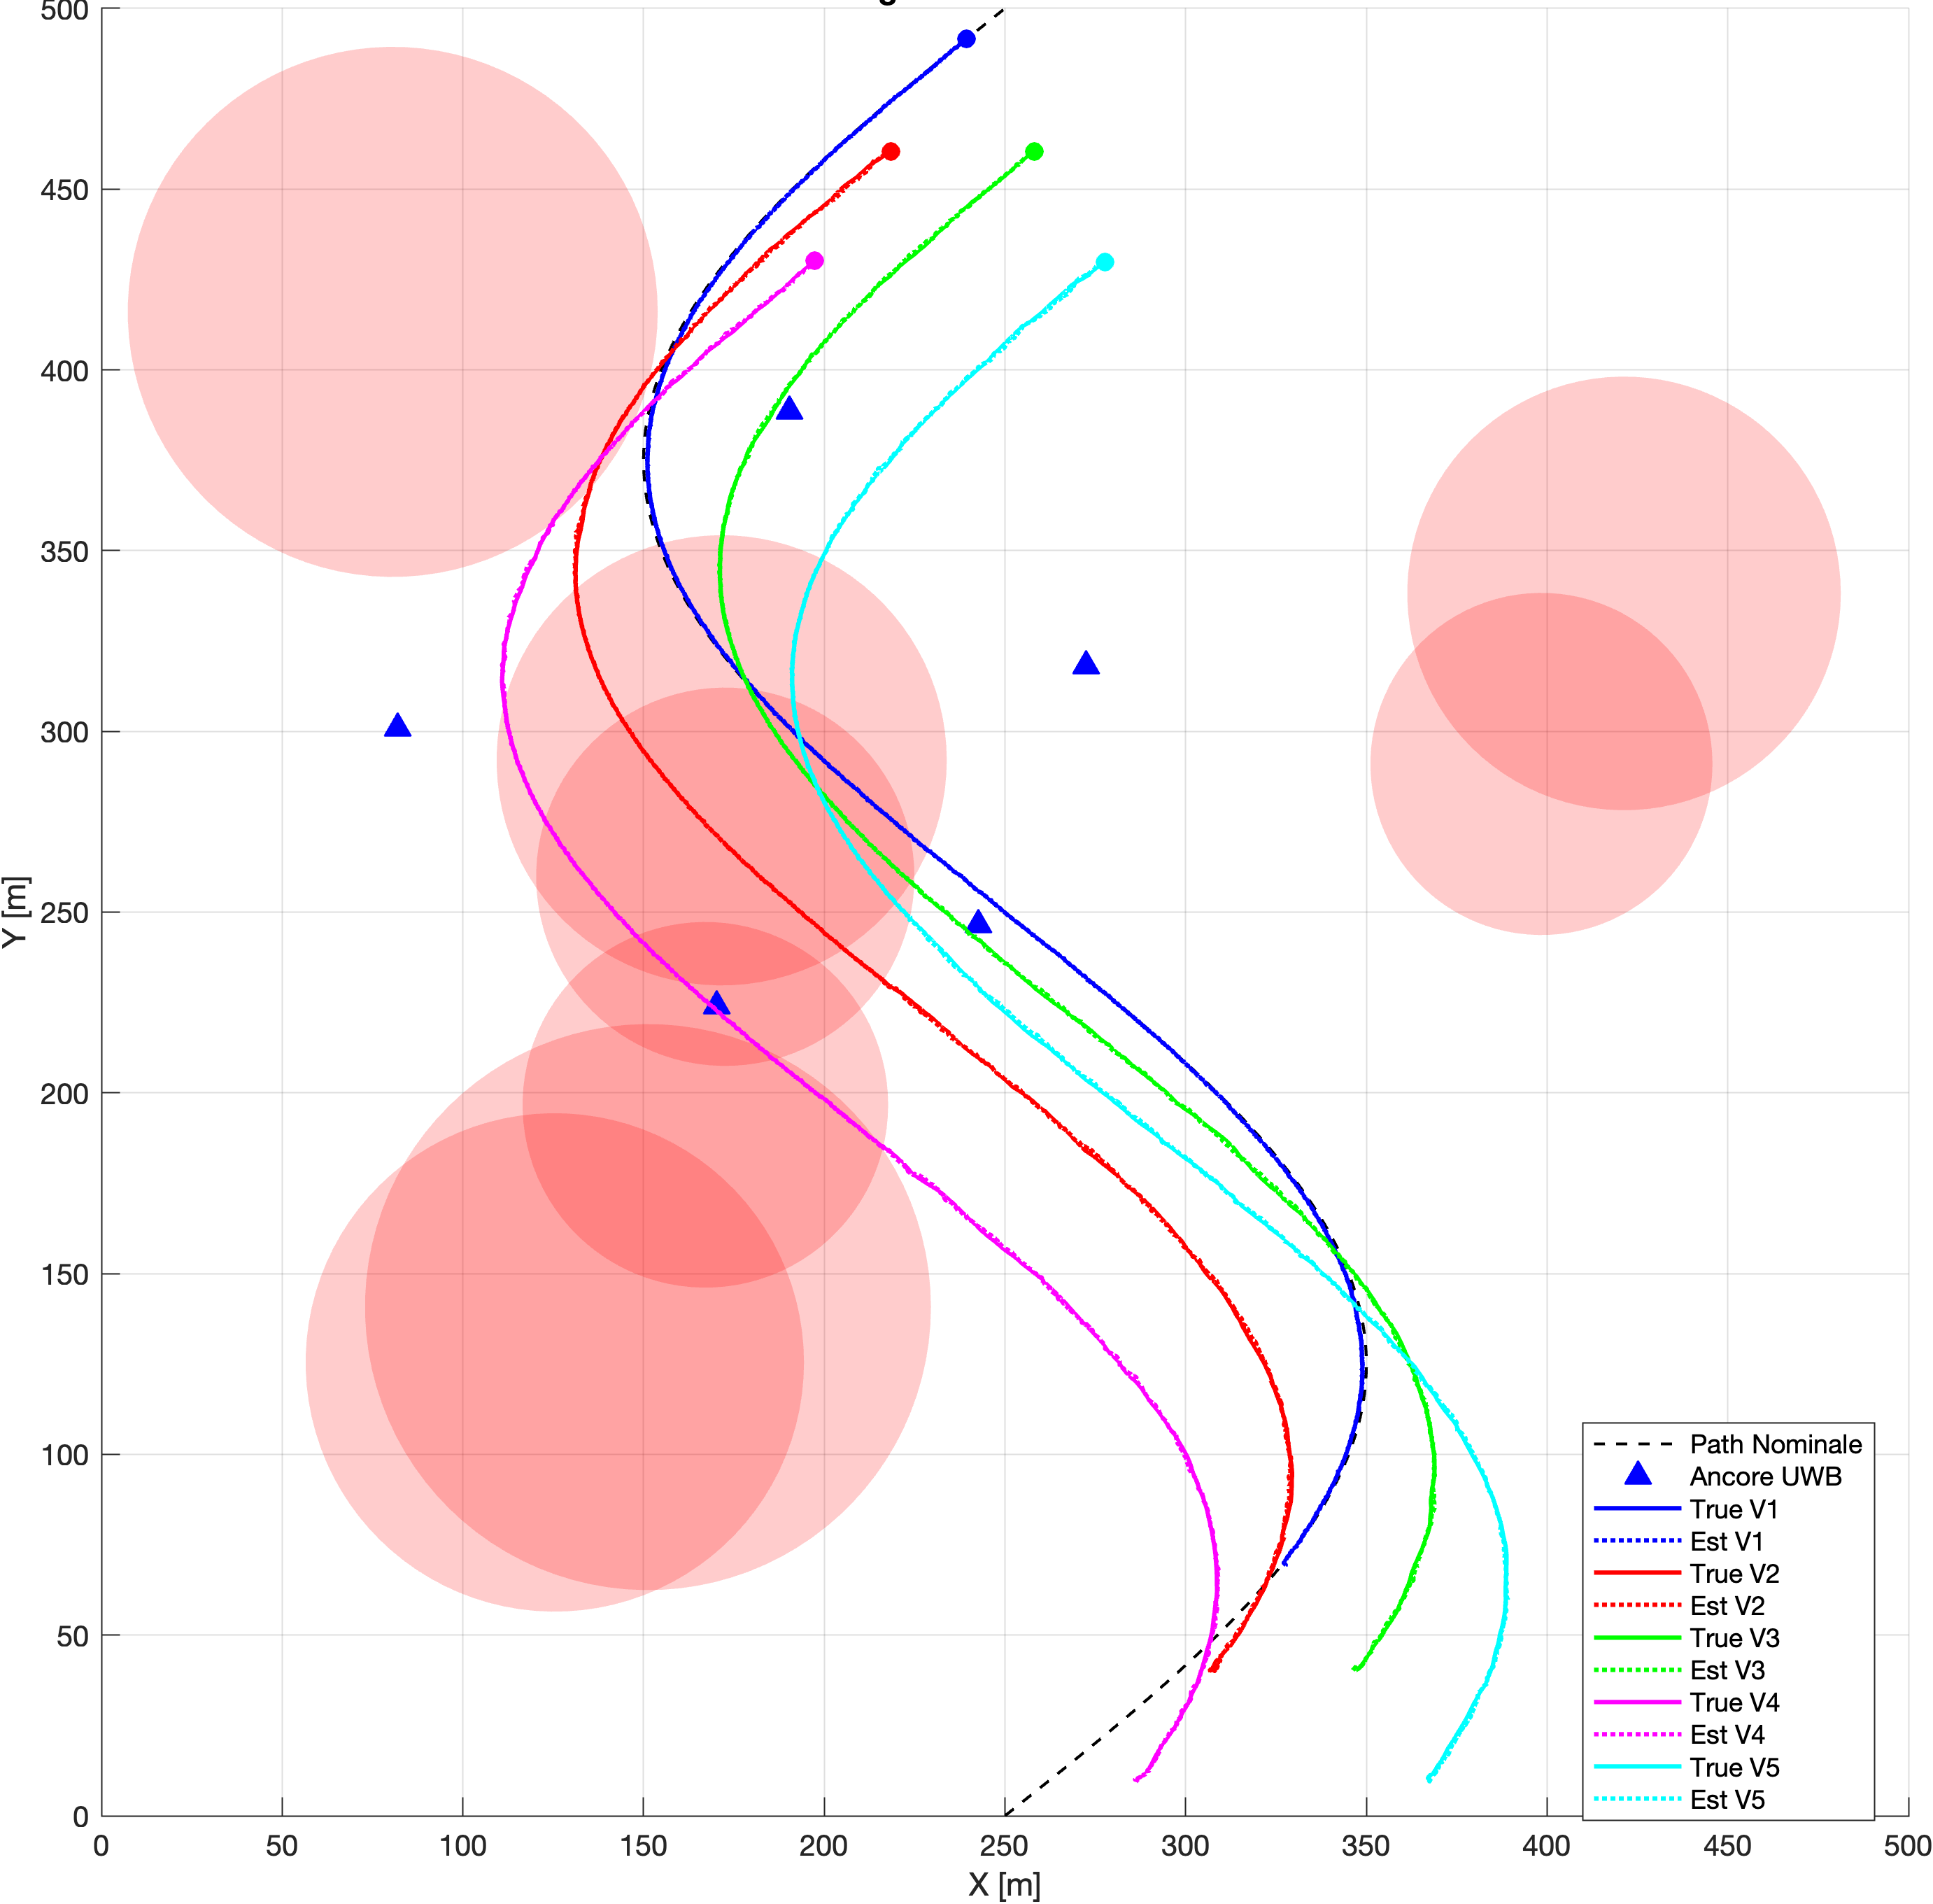
\includegraphics[width=\columnwidth]{figure/1_mappa_navigazione.png}
\caption{Scenario di simulazione. Tratteggio nero: percorso nominale,
inseguito dal solo Master. Cerchi rossi: zone GPS-denied. Triangoli blu: ancore
UWB, collocate per minimizzazione della GDOP. Linee continue: posizione reale
dei cinque veicoli; linee punteggiate: stima dell'EKF. La sovrapposizione fra
le due misura la qualit\`a della localizzazione.}
\label{fig:mappa}
\end{figure}

\subsection{Il grafo di comunicazione diventa un vincolo}

Con $r_{collab} = 55$\,m e la formazione a cinque mezzi, cinque coppie su dieci
non si vedono. La topologia risultante \`e una catena
\texttt{V4--V2--V1--V3--V5} pi\`u l'arco \texttt{V2--V3}: V2 e V3 sono punti di
articolazione, e la caduta di uno dei due staccherebbe un intero ramo. Le
grandezze spettrali sono raccolte in Tab.~\ref{tab:grafo}.

\begin{table}[t]
\centering
\caption{Propriet\`a spettrali del grafo, confronto fra la configurazione a
tre veicoli in grafo completo e quella finale a cinque veicoli.}
\label{tab:grafo}
\begin{tabular}{lrr}
\toprule
\textbf{Grandezza} & \textbf{$N=3$, $K_3$} & \textbf{$N=5$, sparso}\\
\midrule
Archi attivi                       & 3 su 3 & \textbf{5 su 10}\\
Connettivit\`a $\lambda_2(L)$      & 3.000  & \textbf{0.697}\\
Raggio spettrale $\rho_2=|\lambda_2(Q)|$ & 0.000 & \textbf{0.826}\\
Autovalore minimo $\lambda_{min}(Q)$ & 0.000 & $-0.076$\\
Componenti connesse                & 1      & 1\\
Diametro                           & 1 salto & \textbf{3 salti}\\
Guadagno $K_{cons}$                & 0.150  & \textbf{0.646}\\
Costante di tempo $\tau$           & 2.22 s & 2.22 s\\
Margine discretizzazione           & 0.045  & 0.278 (limite 2)\\
Cicli di consenso $q$              & 1      & \textbf{49 su 50}\\
\bottomrule
\end{tabular}
\end{table}

Il salto pi\`u significativo \`e sull'ultima riga. Su grafo completo la regola
di Metropolis d\`a $q_{ij} = 1/N$ per ogni coppia, quindi $\rho_2 = 0$ e il
consenso converge in un solo passo: gli algoritmi di stima distribuita
risultano esatti con una sola iterazione. Con il grafo sparso il
dimensionamento~\eqref{eq:qcicli} richiede \textbf{49 cicli sui 50 disponibili},
cio\`e il 98\% della banda allocata. Il consenso passa da voce marginale a
vincolo di progetto, e la scelta del raggio radio diventa un compromesso fra
qualit\`a del collegamento e costo della comunicazione.

La previsione \`e conservativa: nei fatti ne bastano 34, perch\'e $\rho_2$
governa il decadimento \emph{asintotico} e trascura la costante moltiplicativa.
Sovrastimare \`e il verso giusto in cui sbagliare, ma qui lo si paga in banda.

La Fig.~\ref{fig:grafo} mostra che la topologia resta deterministica per
l'intera missione. Le distanze nominali si separano in due gruppi netti,
36--41\,m e 66--81\,m, con un vuoto di 25\,m in mezzo: il margine \`e del
$+35\%$ sui collegamenti attivi e del $-17\%$ su quelli assenti, quindi
l'errore di formazione non li fa sfarfallare.

\begin{figure*}[t]
\centering
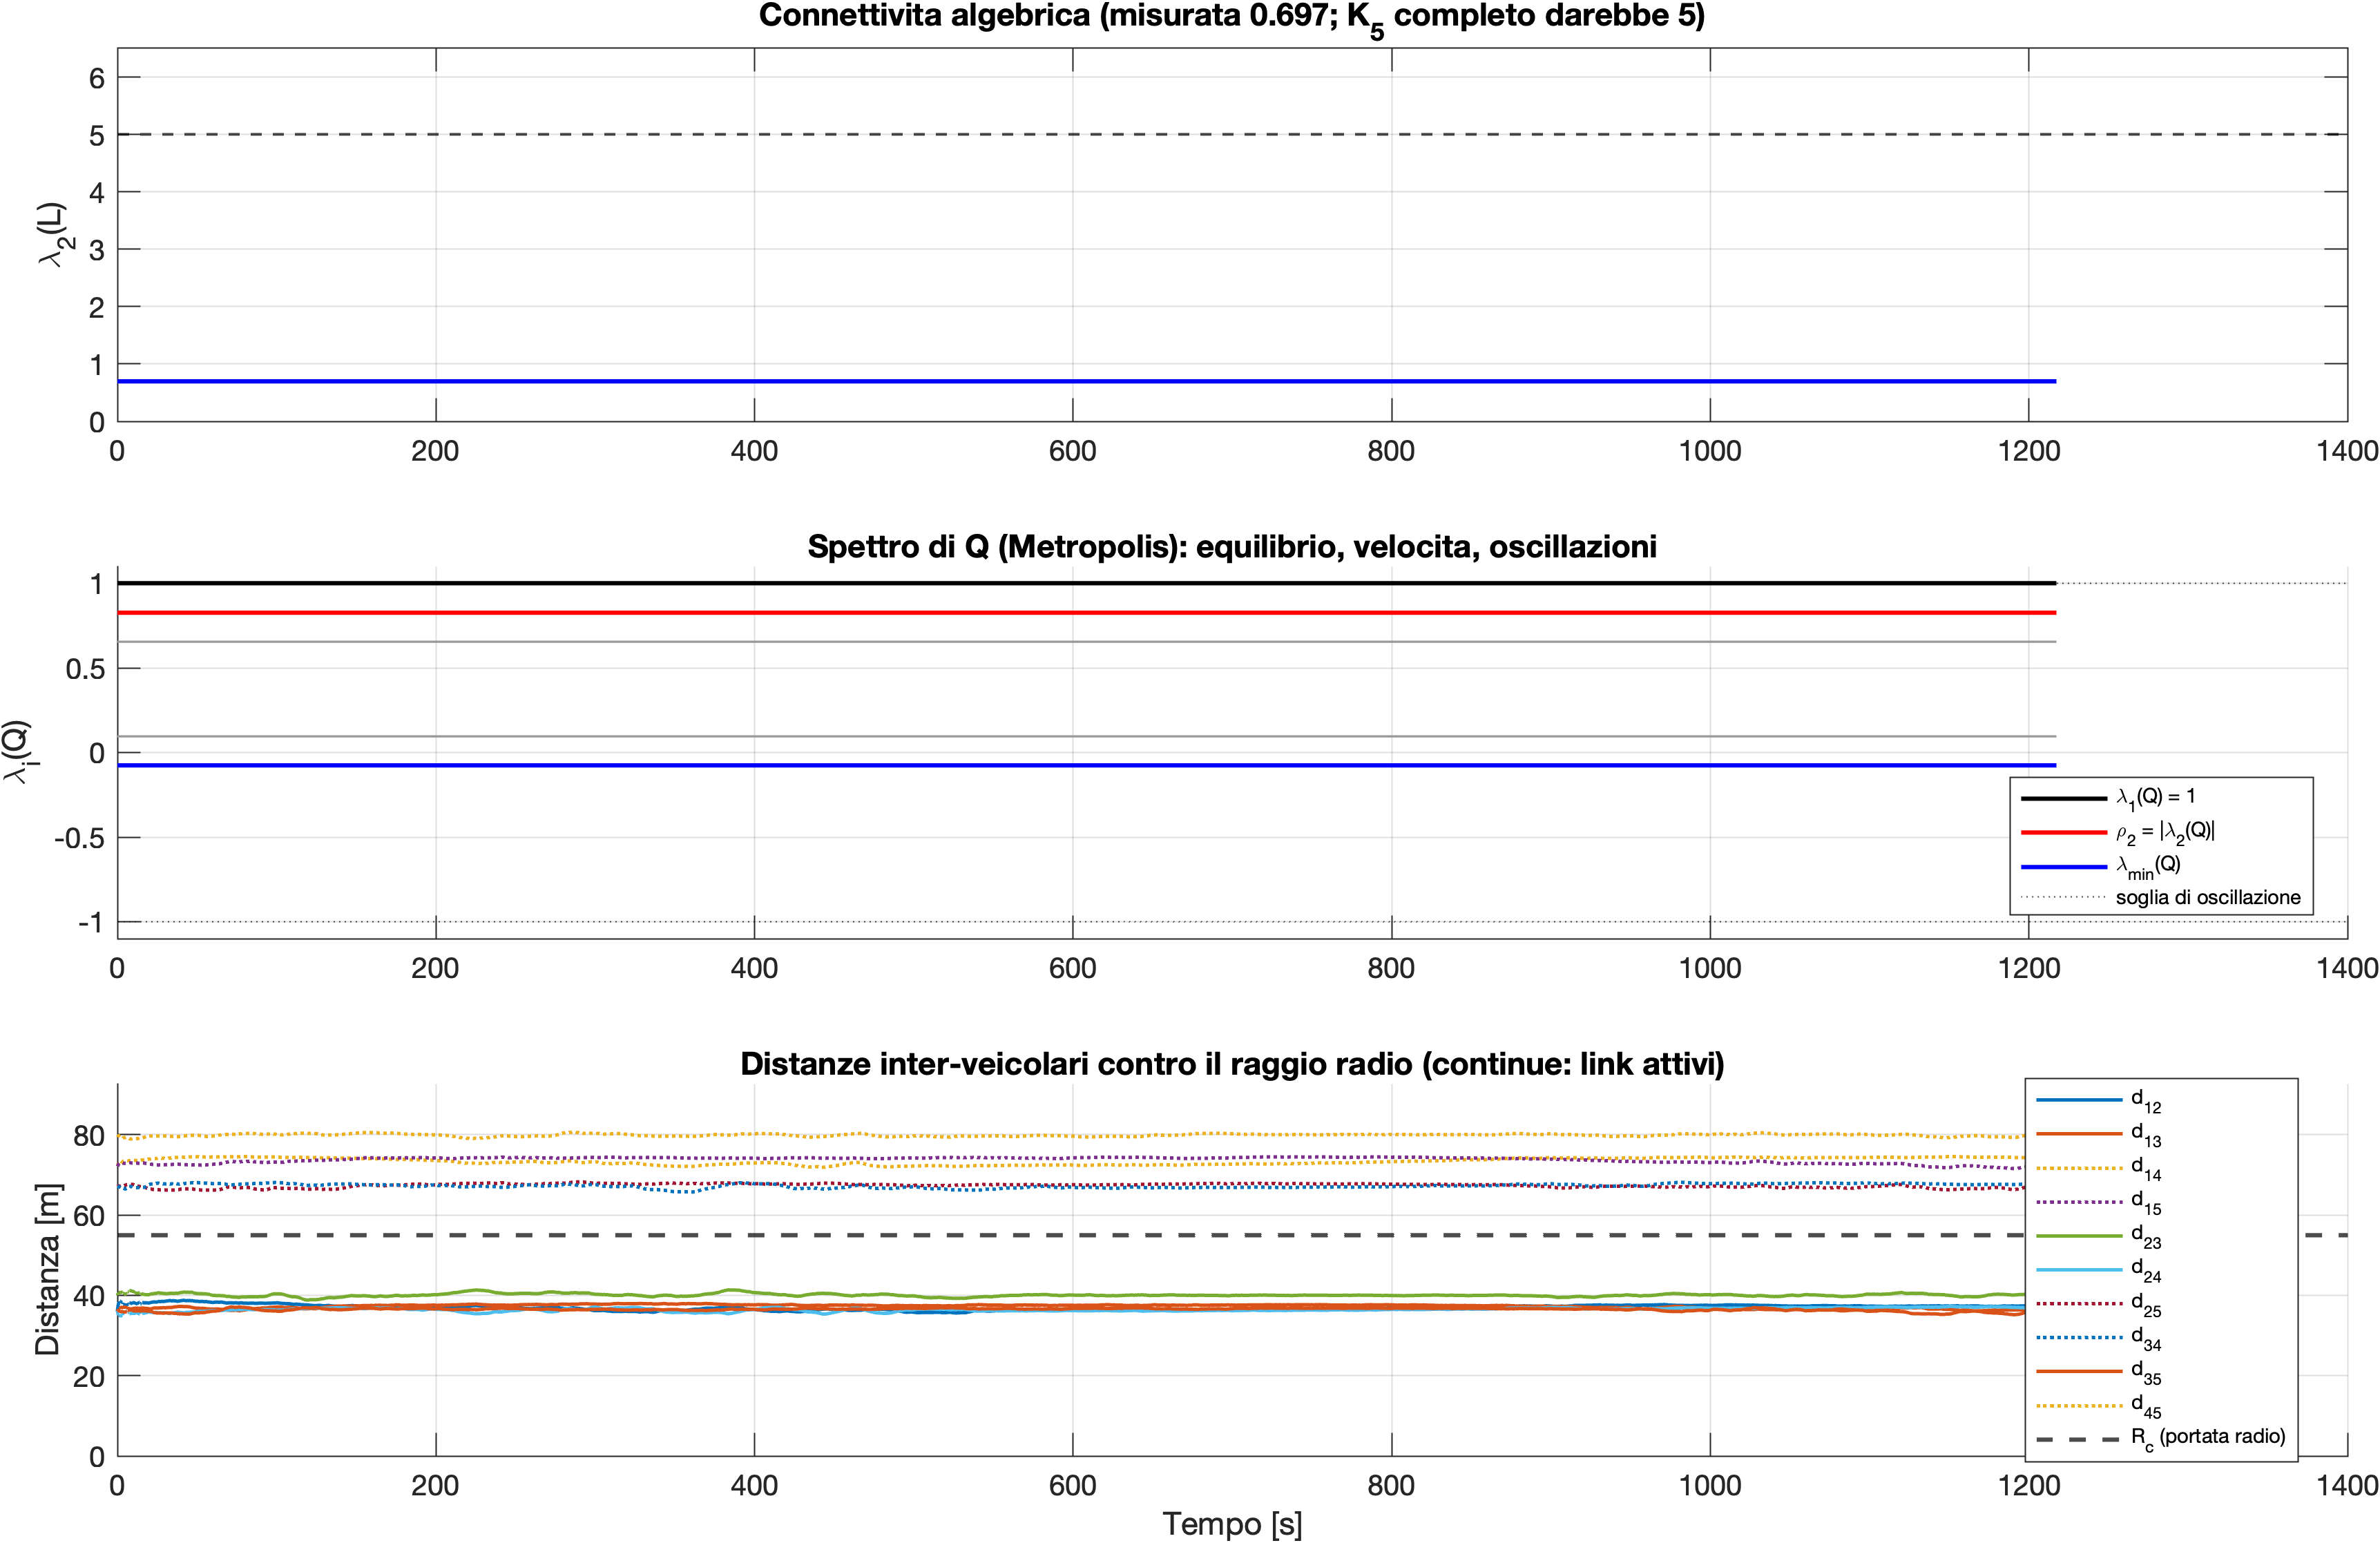
\includegraphics[width=0.86\textwidth]{figure/7_grafo_comunicazione.png}
\caption{Diagnostica del grafo di comunicazione. In alto la connettivit\`a
algebrica $\lambda_2(L)$ e il numero di archi attivi; al centro lo spettro
$\lambda_i(Q)$ della matrice di Metropolis; in basso le dieci distanze
inter-veicolari confrontate con il raggio radio (tratteggio nero). Le cinque
curve continue restano ben sotto la soglia, le cinque punteggiate ben sopra:
\`e il vuoto fra i due gruppi che rende la topologia deterministica malgrado
l'errore di formazione.}
\label{fig:grafo}
\end{figure*}

\subsection{Accuratezza della localizzazione}

La Tab.~\ref{tab:accuratezza} riporta l'errore medio assoluto di posizione,
separato fra tratti con copertura GNSS e tratti in zona cieca.

\begin{table}[t]
\centering
\caption{Errore medio assoluto (MAE) di posizione e traccia della covarianza,
separati per condizione di copertura.}
\label{tab:accuratezza}
\begin{tabular}{lrrr}
\toprule
\textbf{Veicolo} & \textbf{MAE GNSS} & \textbf{MAE cieca} &
$\mathbf{tr(\Sigma_{pos})}$ \textbf{cieca}\\
\midrule
V1 (Master, RTK)  & 0.070 m & 0.078 m & 0.0129 m$^2$\\
V2 (Slave)        & 0.347 m & 0.086 m & 0.0124 m$^2$\\
V3 (Slave)        & 0.332 m & 0.073 m & 0.0131 m$^2$\\
V4 (Slave)        & 0.311 m & 0.084 m & 0.0163 m$^2$\\
V5 (Slave)        & 0.389 m & 0.075 m & 0.0143 m$^2$\\
\bottomrule
\end{tabular}
\end{table}

Il risultato pi\`u vistoso \`e che \textbf{gli Slave stimano quattro volte
meglio in zona GPS-denied che a cielo aperto}. Non \`e un paradosso ma la
conseguenza diretta del confronto fra due fonti di informazione: un ricevitore
NEO-M8N a $\sigma = 2.0$\,m che produce un fix ogni secondo, contro cinque
ancore UWB a $\sigma = 0.5$\,m interrogate a 10\,Hz e geometricamente ben
distribuite. Fra un fix GNSS e l'altro lo Slave passa il 90\% dei passi in sola
predizione, sostenuto da AHRS ed encoder, e l'incertezza cresce.

La Fig.~\ref{fig:covarianza} mostra lo stesso fenomeno sul piano della
covarianza dichiarata, ed \`e il grafico che sintetizza l'intero comportamento
del sistema. Il pannello superiore conta i riferimenti assoluti disponibili a
ciascun veicolo; quello inferiore traccia $\mathrm{tr}(\Sigma_{pos})$ in scala
logaritmica. All'ingresso in zona cieca la traccia \emph{scende} da circa
0.33\,m$^2$ a 0.012\,m$^2$, un \textbf{miglioramento di 27 volte}, e risale
all'uscita. Il Master, che dispone di RTK a 5\,Hz, resta invece pressoch\'e
indifferente: la sua curva \`e la retta orizzontale in basso.

\begin{figure*}[t]
\centering
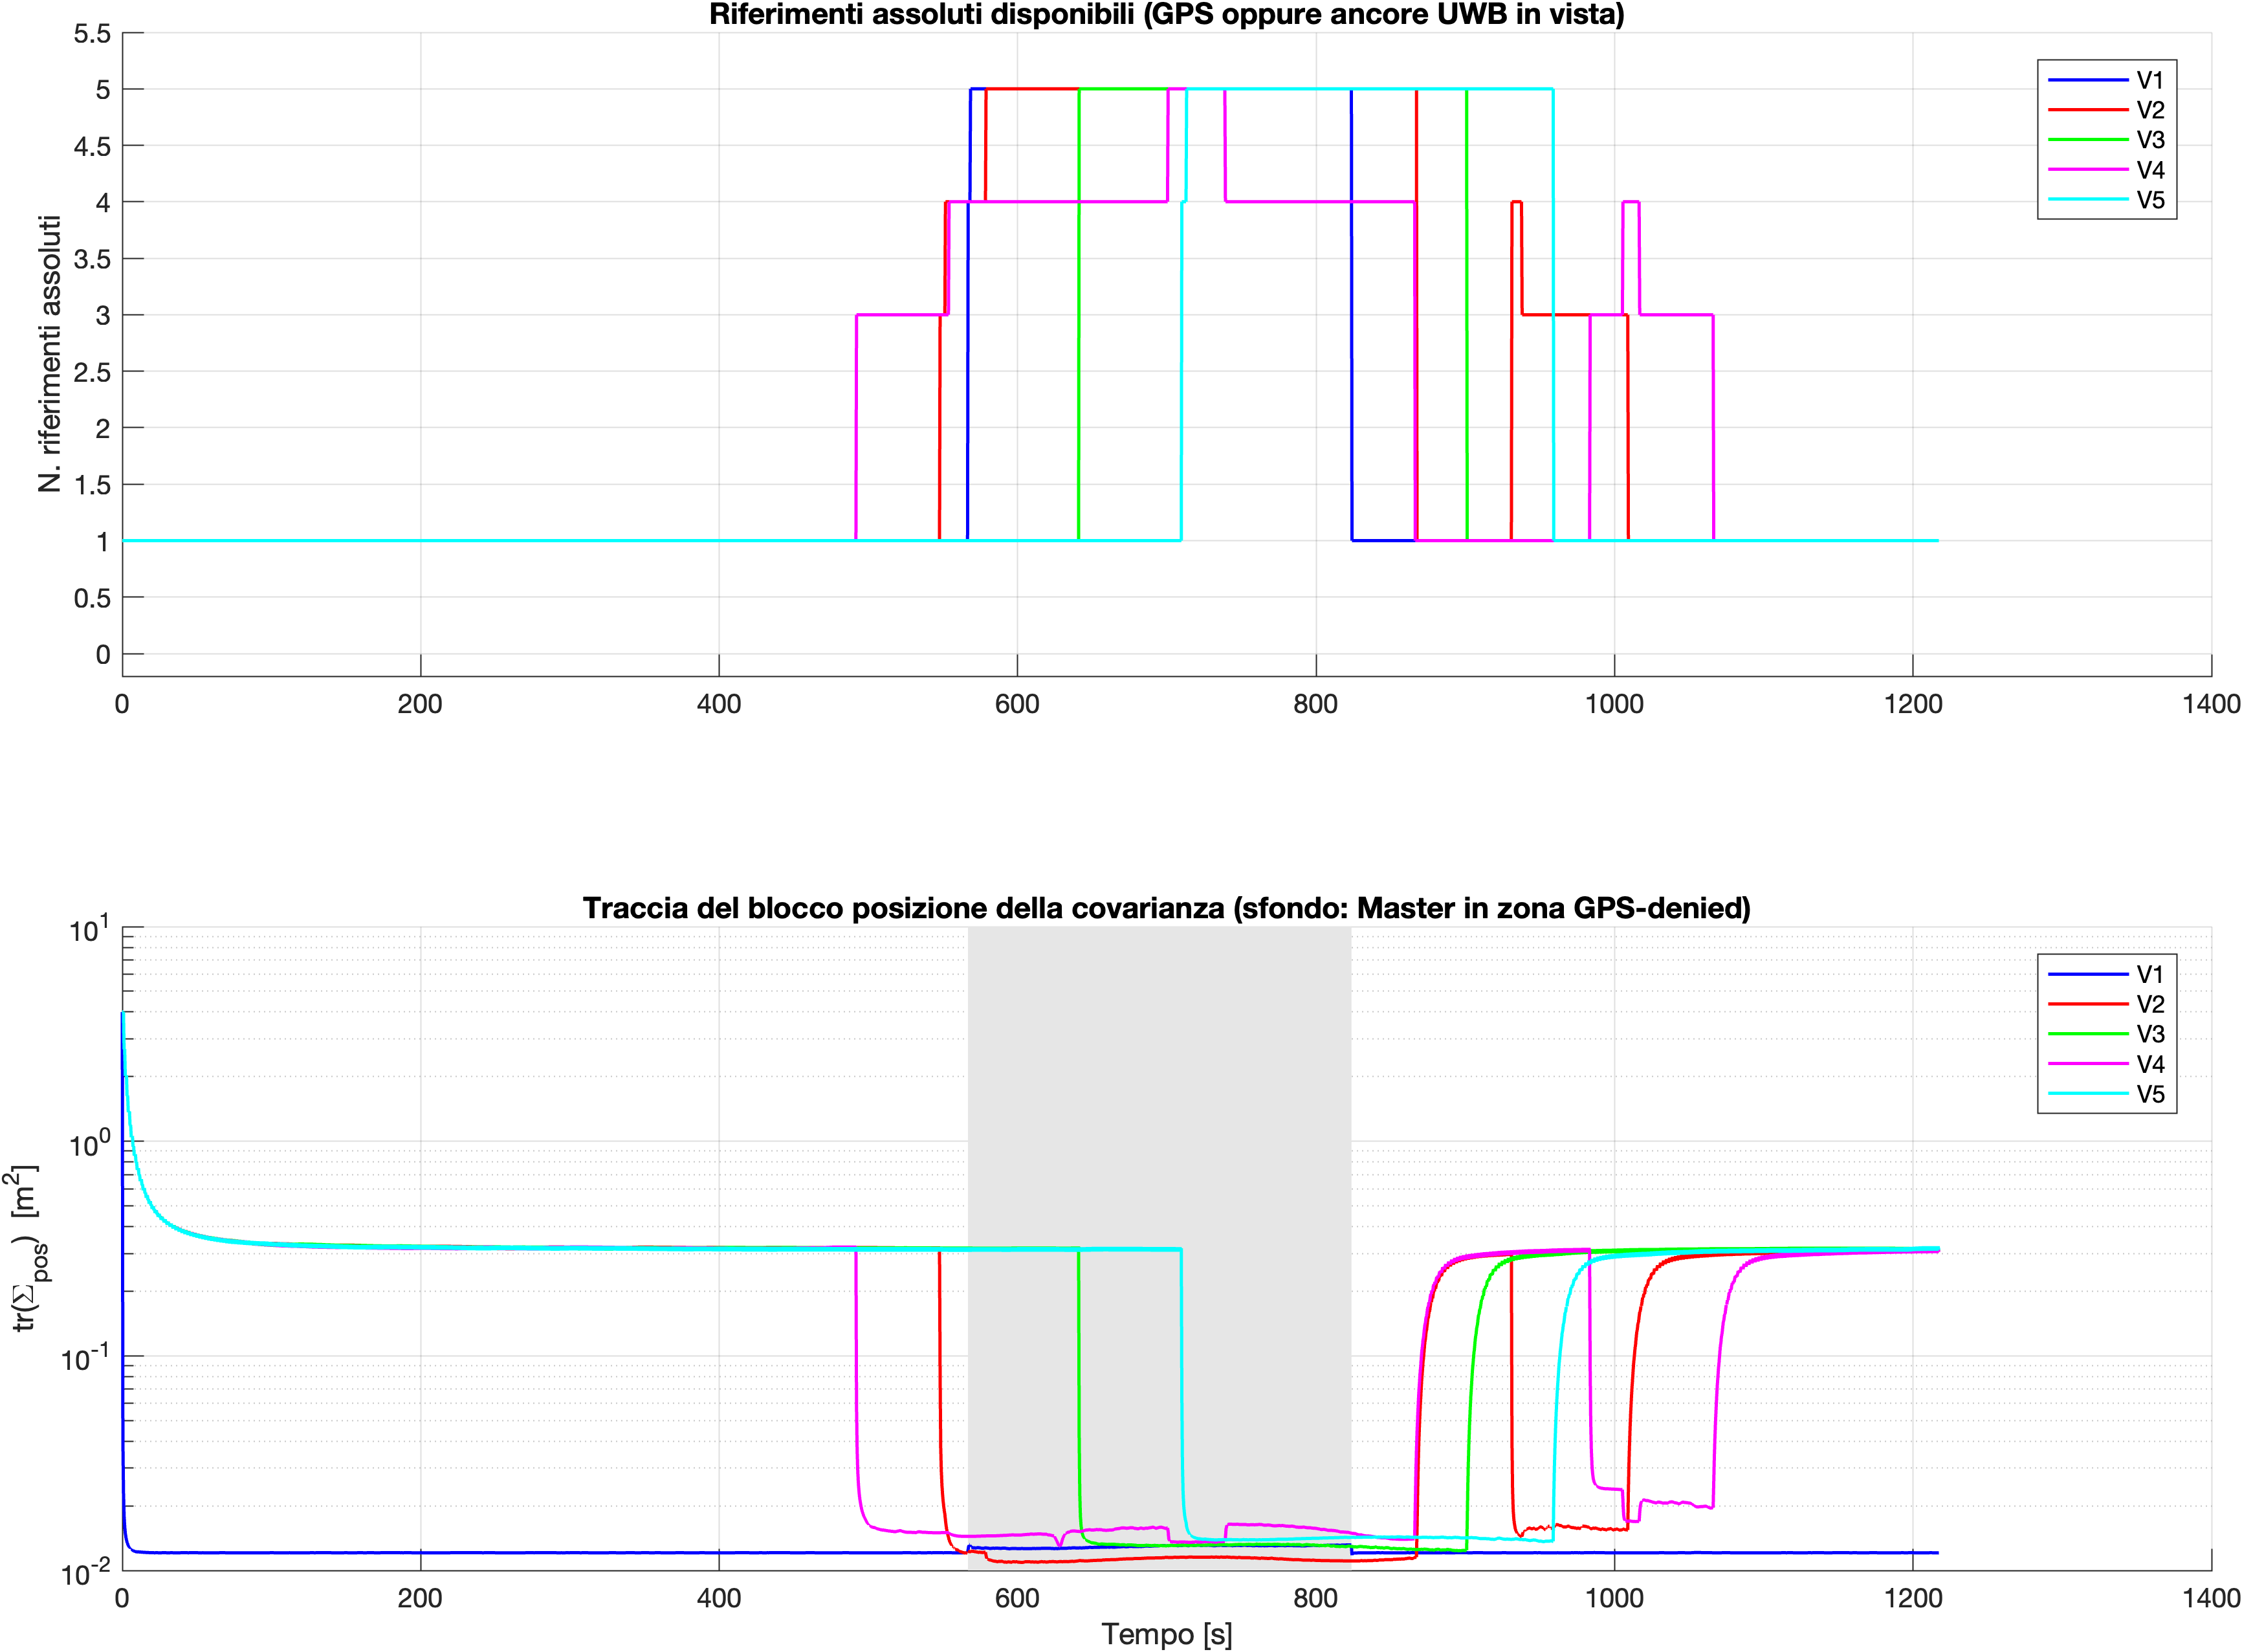
\includegraphics[width=0.86\textwidth]{figure/5_copertura_e_covarianza.png}
\caption{Copertura sensoriale e covarianza. In alto il numero di riferimenti
assoluti (GNSS oppure ancore UWB in vista) per ciascun veicolo; in basso la
traccia del blocco di posizione della covarianza, in scala logaritmica, con
sfondo grigio nei tratti in cui il Master \`e in zona GPS-denied. La discesa di
oltre un ordine di grandezza all'ingresso nella zona cieca \`e il risultato
centrale del lavoro.}
\label{fig:covarianza}
\end{figure*}

Il risultato ha una conseguenza pratica immediata: in un comprensorio
attrezzato con ancore UWB converrebbe fondere UWB e GNSS \emph{simultaneamente}
anzich\'e commutare fra i due, e l'architettura a $C_k$ di dimensione variabile
lo consentirebbe senza modifiche strutturali. \`E discusso in
Sez.~\ref{sec:conclusioni} fra i limiti noti.

Va inoltre osservato che i quattro Slave sono fra loro indistinguibili,
comprese le due ali esterne che hanno un solo vicino ciascuna. Il grafo sparso
non degrada quindi la localizzazione: le ancore fisse restano il riferimento
dominante in zona cieca, e il ranging collaborativo \`e un contributo
aggiuntivo pi\`u che il sostegno principale. La struttura, in cui filtri locali
si scambiano stime per ancorarsi a vicenda, \`e la stessa analizzata
in~\cite{fontanelli2016}.

\subsection{Comportamento del canale}

La Tab.~\ref{tab:canale} riassume il comportamento del collegamento radio.

\begin{table}[t]
\centering
\caption{Canale di comunicazione: valori richiesti e misurati sulla missione
completa (circa 240\,000 tentativi di trasmissione).}
\label{tab:canale}
\begin{tabular}{lr}
\toprule
\textbf{Grandezza} & \textbf{Valore misurato}\\
\midrule
Pacchetti persi                        & 0.48\% (richiesto 0.5\%)\\
Ritardo quantizzato 0 / 1 / 2 passi    & 7\% / 87\% / 7\%\\
Et\`a media del dato usato             & \textbf{100 ms}\\
Et\`a massima del dato usato           & \textbf{400 ms}\\
Margine di stabilit\`a consumato       & 18\% (medio), 71\% (peggiore)\\
Limite teorico~\eqref{eq:ritardo}      & 565 ms\\
Errore dell'ancora mobile              & 0.002 m su $\sigma_{collab}=0.6$ m\\
\bottomrule
\end{tabular}
\end{table}

L'et\`a massima di 400\,ms nasce da due passi di ritardo pi\`u due perdite
consecutive, un evento di probabilit\`a $2.5\cdot10^{-5}$ per coppia e per
passo, che su 240\,000 tentativi si presenta comunque qualche volta. \`E il
caso peggiore e consuma il 71\% del margine~\eqref{eq:ritardo}.

L'effetto misurabile del ritardo \`e sulla \textbf{velocit\`a, non
sull'accuratezza}: la missione si allunga del 13\% (da 1078 a 1218\,s) perch\'e
il consenso agisce su errori di formazione vecchi di 100\,ms, il che equivale a
ridurre il guadagno d'anello. La flotta resta stabile ma reagisce pi\`u
pigramente. Lo 0.5\% di perdita \`e invece praticamente invisibile: alza l'et\`a
media di 0.005 passi, cio\`e mezzo millisecondo.

Un secondo effetto, non legato al canale, riguarda la velocit\`a a regime. Solo
il Master riceve il termine di velocit\`a $V_{rif}$ del path following, mentre
gli Slave si muovono unicamente per consenso. A regime la formazione \`e rigida
e si muove tutta a velocit\`a $v_f$; sommando la~\eqref{eq:consenso} su tutti
gli $i$ e sfruttando $\mathbf{1}^T L = 0$, il termine di consenso sparisce:

\begin{equation}
N\,v_f = \sum_i V_{rif,i} \qquad\Longrightarrow\qquad
v_f = \frac{v_{cruise}}{N}
\label{eq:velflotta}
\end{equation}

Il consenso \`e una forza \emph{interna} e non pu\`o spostare il baricentro:
l'unica spinta esterna viene dal Master e si divide fra tutti. La verifica \`e
esatta: $2.5/3 = 0.83$\,m/s con tre mezzi (misurato 0.83), $2.5/5 = 0.50$ con
cinque (misurato 0.50). Aggiungere veicoli a una formazione del primo ordine
guidata da un Master la rallenta quindi in proporzione diretta. La correzione
\`e di una riga --- propagare $V_{rif}$ a tutta la flotta in avanti --- ed \`e
riportata fra gli sviluppi futuri.

\subsection{Stima distribuita del parametro di terreno}

La flotta esegue un round completo di D-WLS a ogni passo, cio\`e 10\,786 round
sulla missione. La scala dei tempi lo permette: uno scambio UWB dura circa
1\,ms contro i 100\,ms del passo, quindi fra due istanti di controllo il canale
sostiene decine di cicli di consenso. Met\`a del passo \`e riservata a questo
traffico, per un budget di $q_{max} = 50$ cicli.

\begin{table}[t]
\centering
\caption{Validazione numerica del D-WLS. La colonna $K_3$ si riferisce al grafo
completo a tre veicoli, quella sparsa alla configurazione finale.}
\label{tab:dwls_valid}
\begin{tabular}{lrr}
\toprule
\textbf{Propriet\`a verificata} & \textbf{$K_3$} & \textbf{$N=5$ sparso}\\
\midrule
Cicli dimensionati / osservati   & 1 / 1 & 49 / 34\\
Residuo di consenso              & $3.3\cdot10^{-16}$ & $5.5\cdot10^{-6}$\\
Scarto dal WLS centralizzato     & $1.5\cdot10^{-15}$ & $5.2\cdot10^{-7}$\\
Disaccordo fra i veicoli         & $8.4\cdot10^{-16}$ & $9.2\cdot10^{-9}$\\
Invarianza di $\sum_i F_i$       & $2.8\cdot10^{-16}$ & $1.0\cdot10^{-15}$\\
\bottomrule
\end{tabular}
\end{table}

La Tab.~\ref{tab:dwls_valid} confronta la soluzione distribuita con il WLS
centralizzato calcolato lato simulatore. Sul grafo completo l'accordo \`e a
precisione di macchina; sul grafo sparso lo scarto risale a $5\cdot10^{-7}$,
perch\'e con $q$ troncato il consenso \`e \emph{convergente ma non esatto}, che
\`e la condizione normale fuori dal caso completo. L'unica riga che resta a
precisione di macchina \`e l'invarianza della somma $\sum_i F_i$, e questo ha
un significato preciso: le colonne di una matrice doppiamente stocastica
sommano a uno, quindi il consenso \emph{ridistribuisce} l'informazione senza
mai duplicarla. \`E la garanzia che i cicli del grafo non producono doppio
conteggio.

\begin{table}[t]
\centering
\caption{Guadagno della cooperazione sull'incertezza del parametro $c_{terr}$.
L'ultima colonna \`e la dispersione di $v^2$ esplorata da ciascun veicolo.}
\label{tab:dwls_gain}
\begin{tabular}{lrrrr}
\toprule
\textbf{Veicolo} & \textbf{da solo} & \textbf{in rete} & \textbf{guadagno} &
$\mathbf{std(v^2)}$\\
\midrule
V1 (Master)      & $4.55\cdot10^{-4}$ & $4.47\cdot10^{-4}$ & 1.0$\times$ & 0.215\\
V2 (ala interna) & $5.44\cdot10^{-3}$ & $4.47\cdot10^{-4}$ & \textbf{12.2$\times$} & 0.034\\
V3 (ala interna) & $3.13\cdot10^{-3}$ & $4.47\cdot10^{-4}$ & \textbf{7.0$\times$} & 0.070\\
V4 (ala esterna) & $6.74\cdot10^{-3}$ & $4.47\cdot10^{-4}$ & \textbf{15.1$\times$} & 0.017\\
V5 (ala esterna) & $6.33\cdot10^{-3}$ & $4.47\cdot10^{-4}$ & \textbf{14.2$\times$} & 0.020\\
\bottomrule
\end{tabular}
\end{table}

La Tab.~\ref{tab:dwls_gain} quantifica quanto vale la cooperazione. Il confronto
corretto non \`e il numero di condizionamento --- aggiungere Slave lo peggiora
leggermente, pur aggiungendo informazione --- ma la covarianza
$(\sum_i F_i)^{-1}$, che per l'ordinamento di Loewner pu\`o solo ridursi.

L'ultima colonna spiega la terza: il guadagno di ciascun mezzo \`e tanto
maggiore quanto meno quel mezzo, da solo, esplora velocit\`a diverse. Il Master,
che ha sia il torsiometro migliore sia la massima escursione di velocit\`a,
da solo arriverebbe gi\`a dove arriva la rete. \textbf{La rete non produce un
miglioramento uniforme: distribuisce a tutti la qualit\`a del membro meglio
strumentato}, esattamente la stessa struttura del GNSS RTK montato sul solo
Master.

La stima finale vale $\mu_{terr} = 0.0902$ e $c_{terr} = 0.00480$ contro valori
veri di 0.0900 e 0.00500, cio\`e $+1.44$ e $-0.44$ deviazioni standard, con un
errore relativo dello \textbf{0.31\%}. Le due ali esterne, senza cooperare, si
assesterebbero attorno all'8\%. La Fig.~\ref{fig:dwls} mostra l'andamento
temporale: le curve dei cinque veicoli coincidono, mentre le punteggiate
indicano cosa otterrebbe ciascun mezzo da solo.

\begin{figure*}[t]
\centering
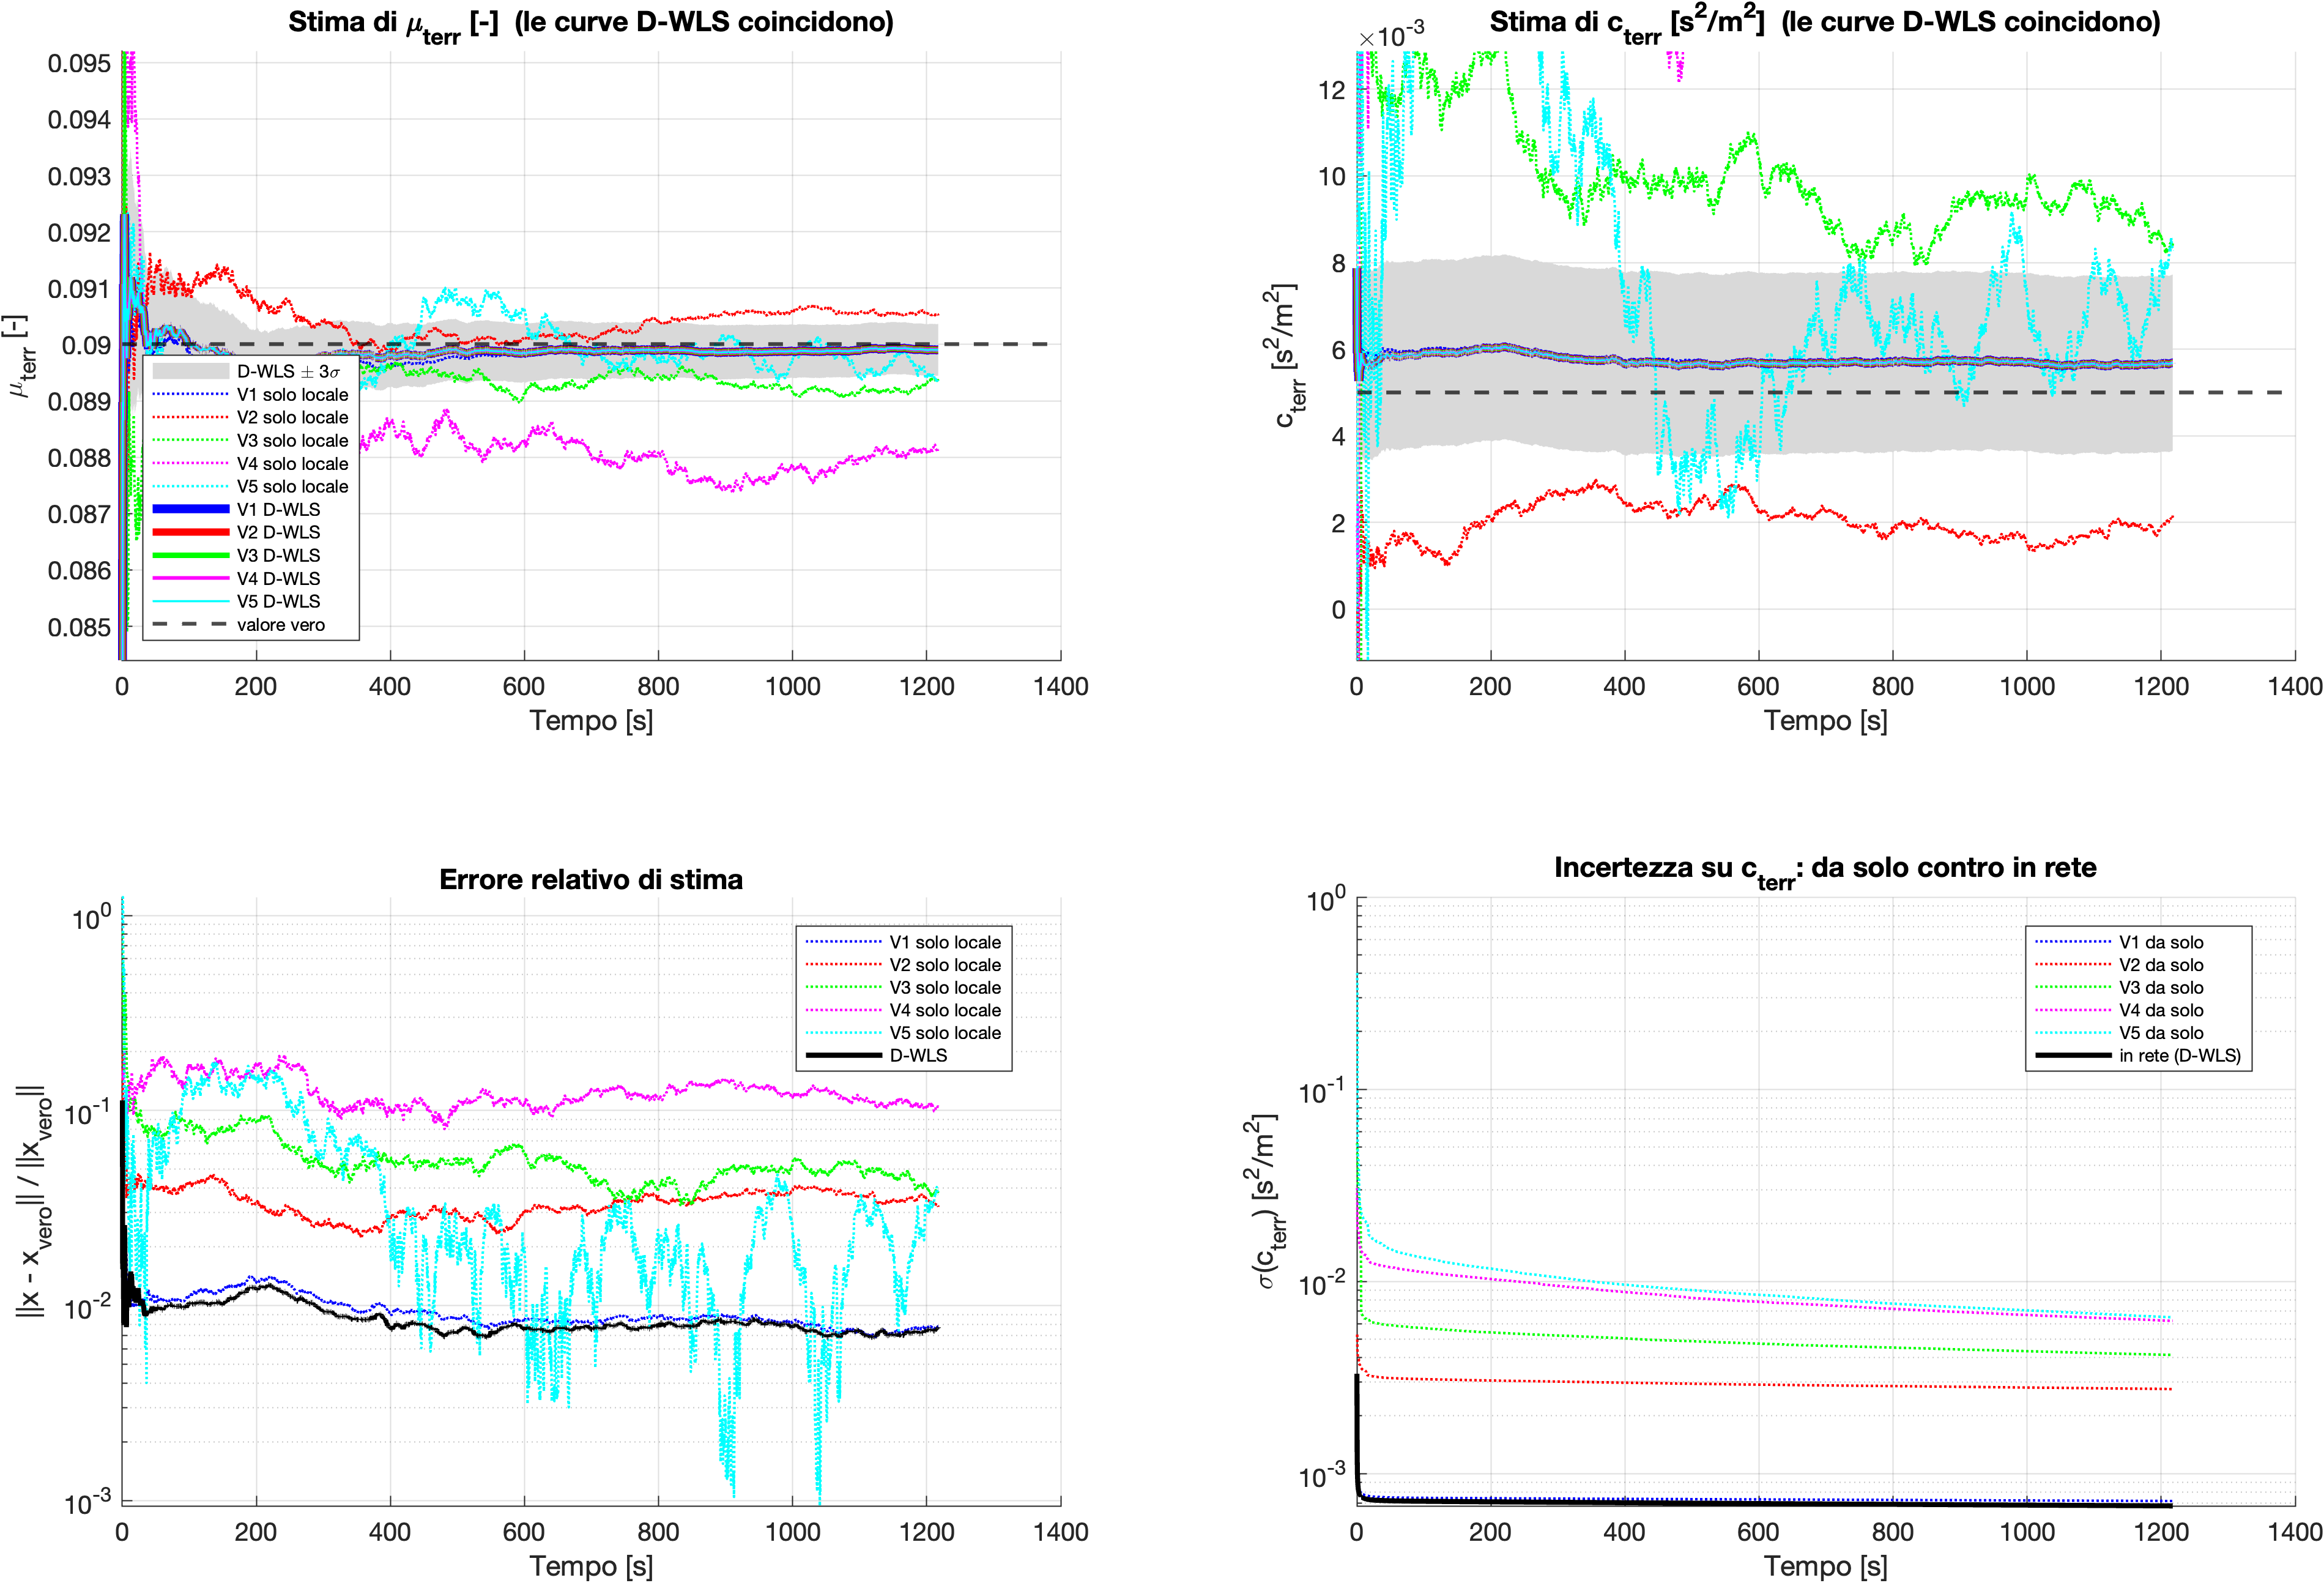
\includegraphics[width=0.86\textwidth]{figure/8_stima_terreno_dwls.png}
\caption{Stima distribuita del parametro di terreno. A sinistra i due parametri
$\mu_{terr}$ e $c_{terr}$ nel tempo: le curve dei cinque veicoli coincidono
(spessore decrescente per distinguerle), le punteggiate mostrano cosa
otterrebbe ciascun mezzo senza cooperare. A destra l'errore relativo e il
guadagno informativo. La convergenza della soluzione distribuita a quella
centralizzata \`e verificata a ogni round.}
\label{fig:dwls}
\end{figure*}

\`E interessante notare che il miglioramento rispetto alla formazione a tre
veicoli (errore relativo dall'1.53\% allo 0.31\%) non viene dall'andare pi\`u
veloci --- la flotta a cinque \`e anzi pi\`u lenta, per
la~\eqref{eq:velflotta} --- ma dall'andare a velocit\`a \emph{pi\`u diverse}.
Le ali esterne stanno a 40\,m dall'asse contro i 20\,m delle interne, quindi in
curva la loro velocit\`a si scosta dal Master il doppio, e cresce la dispersione
di $v^2$ che condiziona il problema di stima. \`E la stessa lezione della GDOP:
conta la diversit\`a geometrica delle misure, non il loro numero.

\subsection{Consistenza del filtro}

Il confronto fra l'errore di stima effettivo e l'inviluppo $\pm 3\sigma$
estratto dalla covarianza dichiarata mostra una frazione di campioni fuori
banda compresa fra 0.0\% e 0.3\%, contro un valore atteso di 0.3\% per un
filtro esattamente calibrato. Il filtro risulta quindi consistente e
leggermente conservativo, che \`e il verso sicuro in cui sbagliare. La verifica
\`e condotta su singolo run a scopo diagnostico: la validazione statistica con
campagna Monte Carlo e test NEES \`e prevista fra gli sviluppi futuri.

%=========================================================================
\section{Conclusioni e sviluppi futuri}
\label{sec:conclusioni}
%=========================================================================

Il lavoro ha portato a un'architettura decentralizzata funzionante per la
localizzazione e il controllo di formazione di una flotta di battipista in
ambiente ostile, validata su un simulatore che include zone GPS-denied,
infrastruttura UWB, grafo di comunicazione non completo, sensori alle loro
frequenze reali e canale con ritardo e perdite.

\subsection{Benefici dimostrati}

\begin{itemize}
\item \textbf{L'infrastruttura UWB compensa pi\`u che sostituire il GNSS.}
      In zona cieca la traccia della covarianza scende di un fattore 27
      rispetto alla navigazione con GNSS di serie a cielo aperto. Cinque ancore
      ben distribuite a $\sigma = 0.5$\,m battono un ricevitore a $\sigma =
      2.0$\,m e 1\,Hz.
\item \textbf{La cooperazione rende risolvibile un problema localmente
      singolare.} Nessun veicolo pu\`o identificare i due parametri di terreno
      da solo, perch\'e la sua matrice di informazione istantanea ha rango 1 su
      2. La rete distribuisce a tutti la qualit\`a del membro meglio
      strumentato, con guadagni fino a 15$\times$ sull'incertezza.
\item \textbf{Le grandezze spettrali sono strumenti di progetto.} La
      connettivit\`a $\lambda_2(L)$ \`e stata usata per dimensionare il guadagno
      di consenso e il raggio spettrale $\rho_2$ per dimensionare il numero di
      cicli di comunicazione, non solo per commentare i risultati.
\item \textbf{La composizione di ritardo e perdite in un'unica grandezza}, cio\`e
      l'et\`a del dato, ha permesso di trattare il canale non ideale senza
      introdurre timestamping n\'e buffer aggiuntivi.
\end{itemize}

\subsection{Limiti noti}

\begin{itemize}
\item \textbf{Il filtro \`e ottimista sulla misura collaborativa.} La matrice
      $R$ associata al ranging fra veicoli contiene il solo rumore del sensore,
      $\sigma_{collab}^2$, e ignora l'incertezza $\Sigma_j$ del vicino, come se
      la sua posa fosse nota esattamente. Il problema pi\`u serio non \`e per\`o
      quello: poich\'e i veicoli si scambiano informazione lungo i cicli del
      grafo, le stime diventano correlate in modo ignoto (\emph{data
      rumination}), e imporre implicitamente correlazione nulla porta a
      sottostimare la covarianza.
\item \textbf{L'architettura a commutazione costa.} Il ramo UWB si attiva
      solo dentro le zone cieche: uno Slave a cielo aperto, nel 90\% dei passi
      in cui non ha un fix GNSS, non usa le ancore anche quando le ha in
      portata, e paga 0.35\,m di errore l\`a dove ne pagherebbe 0.08.
\item \textbf{La formazione rallenta al crescere di $N$}, per
      la~\eqref{eq:velflotta}, perch\'e solo il Master riceve il riferimento di
      velocit\`a.
\item \textbf{Il regressore del D-WLS \`e incerto.} La riga
      $C_i = [1\ \ \hat v_i^2]$ usa la velocit\`a stimata, l'unica disponibile a
      bordo, e un regressore rumoroso attenua la pendenza verso lo zero
      (\emph{errors-in-variables}). Rifacendo il calcolo con la velocit\`a vera
      si ottiene $c_{terr} = 0.005015$, cio\`e $+0.03$ deviazioni: l'effetto
      esiste ma \`e piccolo rispetto all'informazione disponibile.
\item \textbf{L'aderenza \`e ideale.} La velocit\`a reale coincide istante per
      istante con quella comandata, il che \`e proprio l'ipotesi meno
      difendibile per un mezzo cingolato su neve.
\end{itemize}

\subsection{Sviluppi futuri}

Il lavoro prosegue lungo due direzioni gi\`a individuate.

\textbf{Fusione consistente tramite Covariance Intersection.} \`E la risposta
al primo limite elencato. La CI \cite{julier1997} fonde due stime pesandone le
inverse delle covarianze con $\gamma$ e $1-\gamma$, e garantisce una covarianza
che maggiora quella reale \emph{per qualunque} correlazione incrociata, senza
doverla conoscere:
\begin{equation}
\Sigma^{-1} = \gamma\,\bar\Sigma^{-1} + (1-\gamma)\,C^T R^{-1} C
\label{eq:ci}
\end{equation}
dove $\gamma \in [0,1]$ \`e scelto minimizzando una misura della dimensione di
$\Sigma$. La CI classica non si applica per\`o direttamente al caso in esame:
fonde due stime della \emph{stessa} grandezza, mentre qui il vicino trasmette
una stima del \emph{proprio} stato, e da una misura di sola distanza non si
ricava una stima puntuale della propria posizione. La formulazione corretta
\`e quella di Carrillo-Arce \emph{et al.} \cite{carrillo2013}, in cui
l'incertezza del vicino entra proiettata sulla direzione della congiungente.
Va sottolineato che l'intervento richiede anche di estendere il pacchetto
scambiato dalla sola posizione alla coppia
$(\hat p_j, \Sigma_j^{(1:2,1:2)})$, e che le due modifiche vanno introdotte
\emph{insieme}: usare $\Sigma_j$ per gonfiare $R$ lasciando il guadagno di
Kalman standard tratterebbe l'incertezza del vicino come rumore
\emph{indipendente}, che \`e proprio il doppio conteggio da evitare.

\textbf{Modellazione dello slittamento.} La ground truth passerebbe da
$v^{true} = v^{cmd}$ a una legge $v^{true} = f_{slip}(v^{cmd}, x^{true},
\text{terreno})$, con tre conseguenze a cascata: il modello di misura degli
encoder~\eqref{eq:enc} si carica di un errore \emph{sistematico} (gli encoder
misurano la velocit\`a dei cingoli, non quella del veicolo, e un bias non \`e
rumore bianco); il rumore di processo va ritarato attivando la legge adattiva
$q_a(v) = q_{a0} + k_{terreno}\,v^2$; e il parametro di terreno identificato
dal D-WLS diventa l'ingresso naturale di quella taratura, dato che la stessa
struttura $\mu + c\,v^2$ che descrive la resistenza al moto governa la
dipendenza dello slittamento dalla velocit\`a.

Restano inoltre da affrontare la validazione statistica con campagna Monte
Carlo e test NEES, e il regime di perdite elevate in cui la topologia si
frammenta davvero e il grafo va riletto in termini di \emph{connettivit\`a
congiunta}: la rete pu\`o essere disconnessa a ogni singolo istante e sostenere
ugualmente il consenso, purch\'e nel tempo i collegamenti coprano l'intera
flotta.

\balance

%=========================================================================
\begin{thebibliography}{9}

\bibitem{fontanelli_notes}
D.~Fontanelli, \emph{Intelligent Distributed Systems --- Course Notes},
Universit\`a degli Studi di Trento, 2024/2025.

\bibitem{thrun2005}
S.~Thrun, W.~Burgard, and D.~Fox, \emph{Probabilistic Robotics}.
Cambridge, MA: MIT Press, 2005.

\bibitem{barshalom2001}
Y.~Bar-Shalom, X.~R.~Li, and T.~Kirubarajan, \emph{Estimation with
Applications to Tracking and Navigation}. New York: Wiley, 2001.

\bibitem{olfati2004}
R.~Olfati-Saber and R.~M.~Murray, ``Consensus problems in networks of agents
with switching topology and time-delays,'' \emph{IEEE Trans. Automat. Contr.},
vol.~49, no.~9, pp.~1520--1533, Sep.~2004.

\bibitem{xiao2004}
L.~Xiao and S.~Boyd, ``Fast linear iterations for distributed averaging,''
\emph{Systems \& Control Letters}, vol.~53, no.~1, pp.~65--78, 2004.

\bibitem{khatib1986}
O.~Khatib, ``Real-time obstacle avoidance for manipulators and mobile
robots,'' \emph{Int. J. of Robotics Research}, vol.~5, no.~1, pp.~90--98, 1986.

\bibitem{julier1997}
S.~J.~Julier and J.~K.~Uhlmann, ``A non-divergent estimation algorithm in the
presence of unknown correlations,'' in \emph{Proc. American Control
Conference}, Albuquerque, NM, 1997, pp.~2369--2373.

\bibitem{carrillo2013}
L.~C.~Carrillo-Arce, E.~D.~Nerurkar, J.~L.~Gordillo, and S.~I.~Roumeliotis,
``Decentralized multi-robot cooperative localization using covariance
intersection,'' in \emph{Proc. IEEE/RSJ Int. Conf. on Intelligent Robots and
Systems (IROS)}, Tokyo, Japan, 2013, pp.~1412--1417.

\bibitem{fontanelli2016}
D.~Fontanelli, D.~Macii, P.~Nazemzadeh, and L.~Palopoli, ``Collaborative
Localization of Robotic Wheeled Walkers using Interlaced Extended Kalman
Filters,'' in \emph{Proc. IEEE Int. Instrumentation and Measurement Technology
Conference (I2MTC)}, Taipei, Taiwan, May 2016, pp.~1--6.

\end{thebibliography}

\end{document}
